%!TEX root = Thesis.tex

\chapter{Experimental Results}
\label{cha:experimental_results}

Through the course of this work, we make extensive use three core components:
visual car detection, parking lot modeling and planning. In this section, we
present the experimental evaluation of each of these parts.

\section{Visual Car Detection}
\label{sec:visual_car_detection}

We start the visual detection section by describing the dataset that we
utilize to train the car detector. A training dataset plays a crucial part in
any detection algorithm. In order to train the visual car detector we assemble
a training dataset that consists of a number of positive (containing cars) and
negative (images not containing cars) examples.

\begin{figure}[b]%
\centering
\subfloat{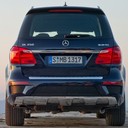
\includegraphics[width=0.14\textwidth]{pictures/pos_1.png}}
\hspace{2mm}
\subfloat{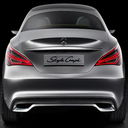
\includegraphics[width=0.14\textwidth]{pictures/pos_2.png}}
\hspace{2mm}
\subfloat{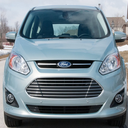
\includegraphics[width=0.14\textwidth]{pictures/pos_3.png}}
\hspace{2mm}
\subfloat{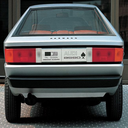
\includegraphics[width=0.14\textwidth]{pictures/pos_4.png}}
\hspace{2mm}
\subfloat{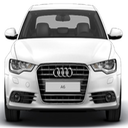
\includegraphics[width=0.14\textwidth]{pictures/pos_5.png}}
\hspace{2mm}
\subfloat{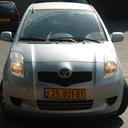
\includegraphics[width=0.14\textwidth]{pictures/pos_6.png}}\\
\subfloat{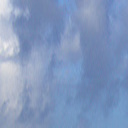
\includegraphics[width=0.14\textwidth]{pictures/neg_1.jpg}}
\hspace{2mm}
\subfloat{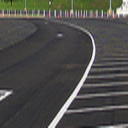
\includegraphics[width=0.14\textwidth]{pictures/neg_2.jpg}}
\hspace{2mm}
\subfloat{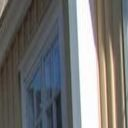
\includegraphics[width=0.14\textwidth]{pictures/neg_3.jpg}}
\hspace{2mm}
\subfloat{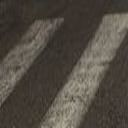
\includegraphics[width=0.14\textwidth]{pictures/neg_4.jpg}}
\hspace{2mm}
\subfloat{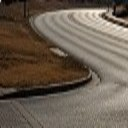
\includegraphics[width=0.14\textwidth]{pictures/neg_5.jpg}}
\hspace{2mm}
\subfloat{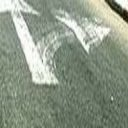
\includegraphics[width=0.14\textwidth]{pictures/neg_6.jpg}}
\caption{Examples of positive and negative training examples for front/rear car detector.}
\label{fig:pos_neg_examples}
\end{figure}

For the reason that the car's view depends on the angle of view, we assemble
positive training data for different angles of the cars. We prepare training
samples for four distinct views of the cars --- front, back and both left and
right sides.

The sides of the car are invariant under the mirror transformation. This
allows to use the same image for training a classifier for each side which
simplifies the training data generation. Front and back of the car, though
different to human point of view, seem to be similar in the HOG visualization.
Therefore, the corresponding datasets can be combined into one.

These datasets contain respectively images of sizes $128 \times 128$ pixels
for front/rear car view and $128 \times 64$ pixels for side view. We utilize
682 positive images that contain cars for training the front/rear detector. In
addition to these positive examples we also convene 7972 negative images. Some
examples from the front/rear positive and negative training datasets are
presented in Figure~\ref{fig:pos_neg_examples}.

The positive examples contain exclusively views of the cars. Each positive
example shows one and only one car. The car occupies the full area of the
image. The photos of the cars depict them centered and seen from the same
angle of view. This is crucial for training a meaningful classifier.

The positive dataset is assembled from different sources: INRIA Car Dataset
by~\citet{inriadata}, Motorway Car Dataset by~\citet{TMEMotorwayDataset}, UIUC
Image Database for Car Detection by~\citet{agarwal2002uiuc}, KITTI car dataset
by~\citet{Geiger2013IJRR} and various car images found in a public domain via
a web searching engine.

In order to create the negative set we randomly sample different sized patches
of the given aspect-ratio ($128 \times 128$ and $128 \times 64$ respectively)
from the images that contain no cars. Following the work of~\citet{dalal2005}
we cut false detections that appear in the first runs of training the
classifier with a clipping tool~\cite{imageclipper} and add them to the
negative training dataset.

We use the trained classifier on the images from the camera mounted inside of
the car facing sidewards or, possibly, onto any other moving platform. During
our experiments we use a Bumblebee stereo-camera
(Figure~\ref{subfig:bumblebee}) pointed to the side of the Europa robot Obelix
(Figure~\ref{subfig:obelix}).

\begin{figure}[t]%
\centering
\subfloat{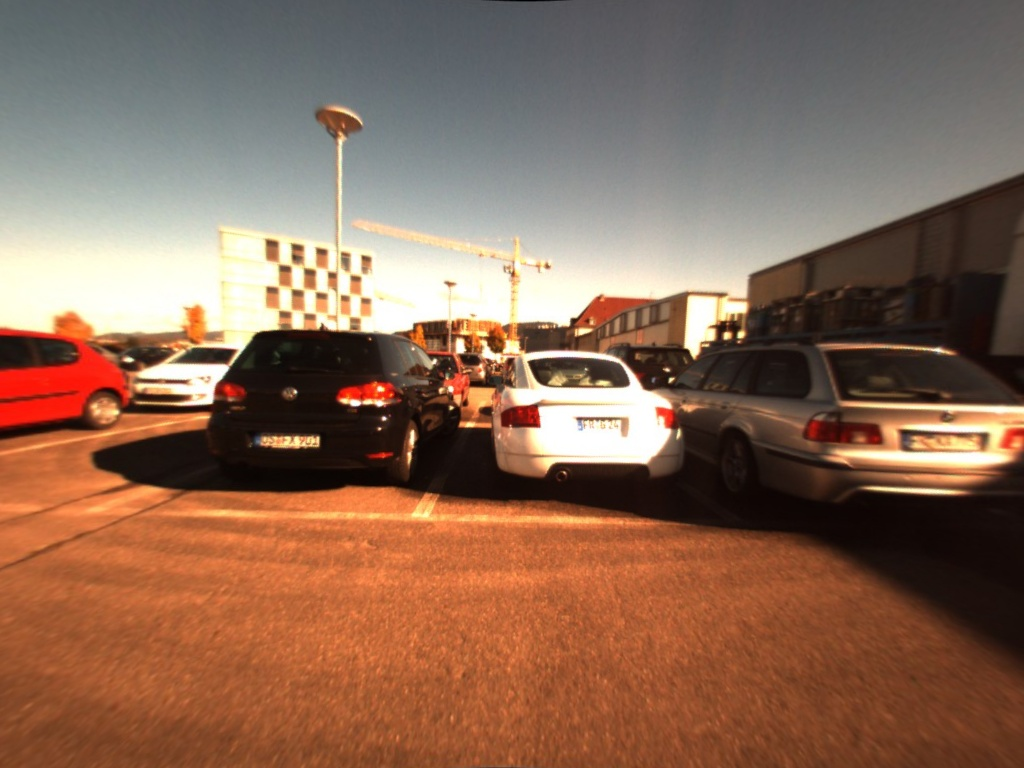
\includegraphics[width=0.31\textwidth]{pictures/left.jpg}}\hspace{2mm}
\subfloat{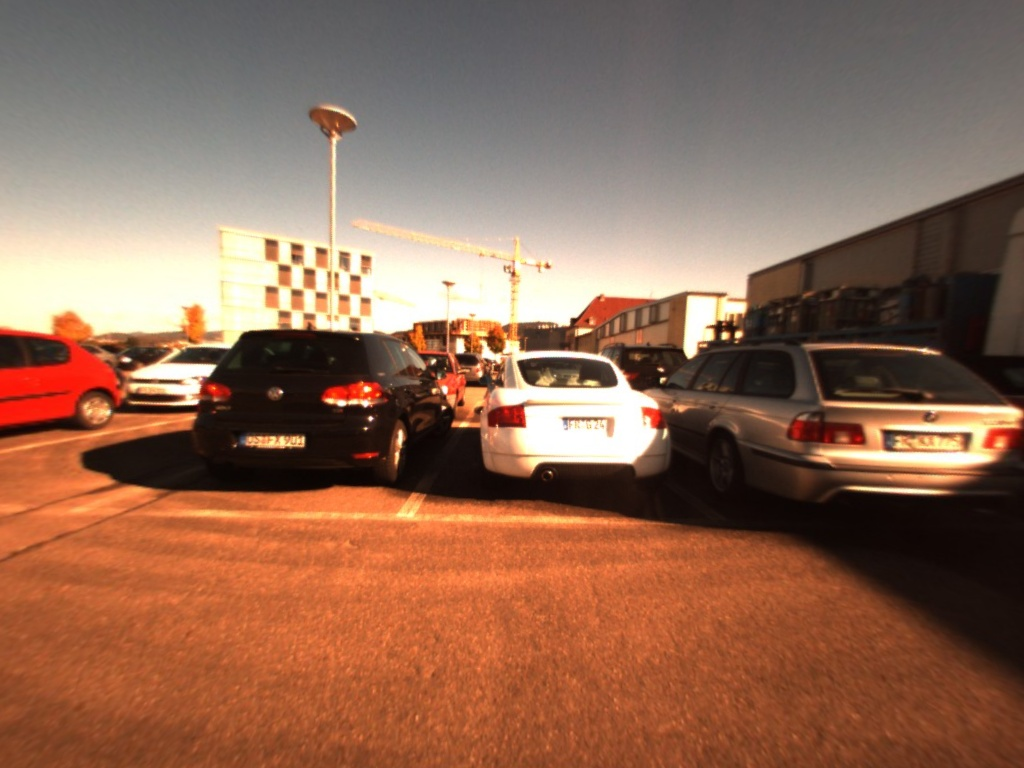
\includegraphics[width=0.31\textwidth]{pictures/right.jpg}}\hspace{2mm}
\subfloat{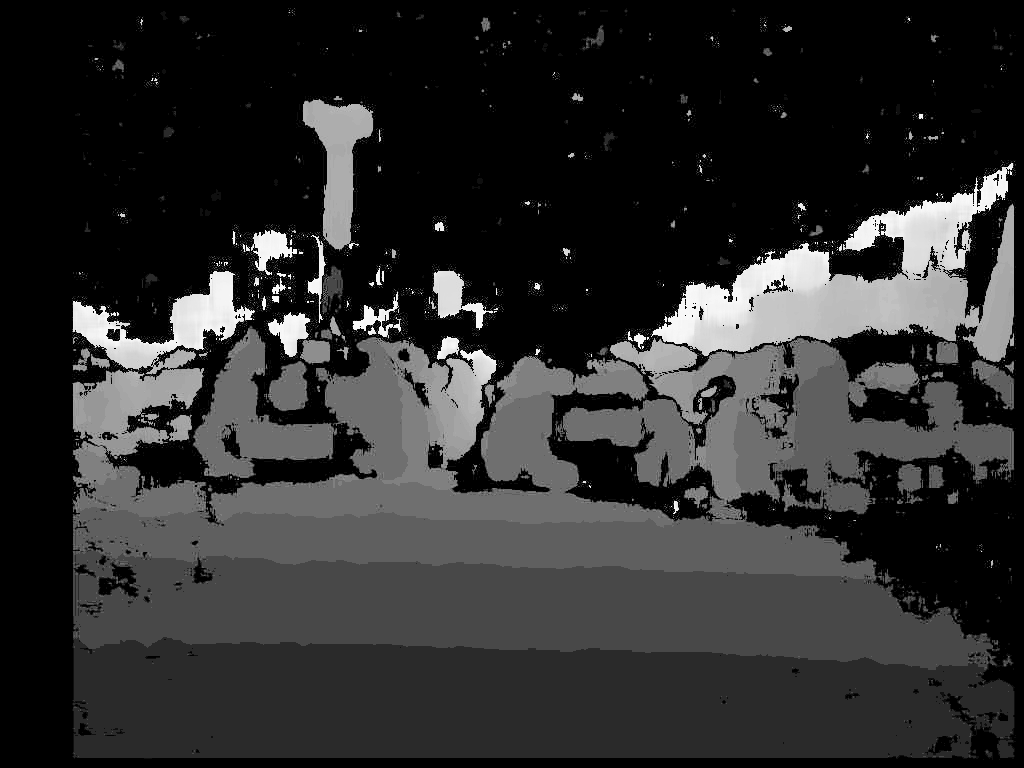
\includegraphics[width=0.31\textwidth]{pictures/depth.png}}\\
\caption{Depth acquired from disparity between stereo images.}
\label{fig:depth_from_disparity}
\end{figure}

We are interested in detections accumulated over time. The same car is seen
from different angles, throughout different (usually consequent) images. We
consider the car to be detected if it has been detected at least once in the
sequence of images, featuring this particular car. With this in mind, the
detection rate for our realization of the approach is approximately 95\%.

The examples of detected cars can be seen in
Figure~\ref{fig:detection_examples}.

\begin{figure}[t]
\centering
\begin{tabular}{cc}
\subfloat[]{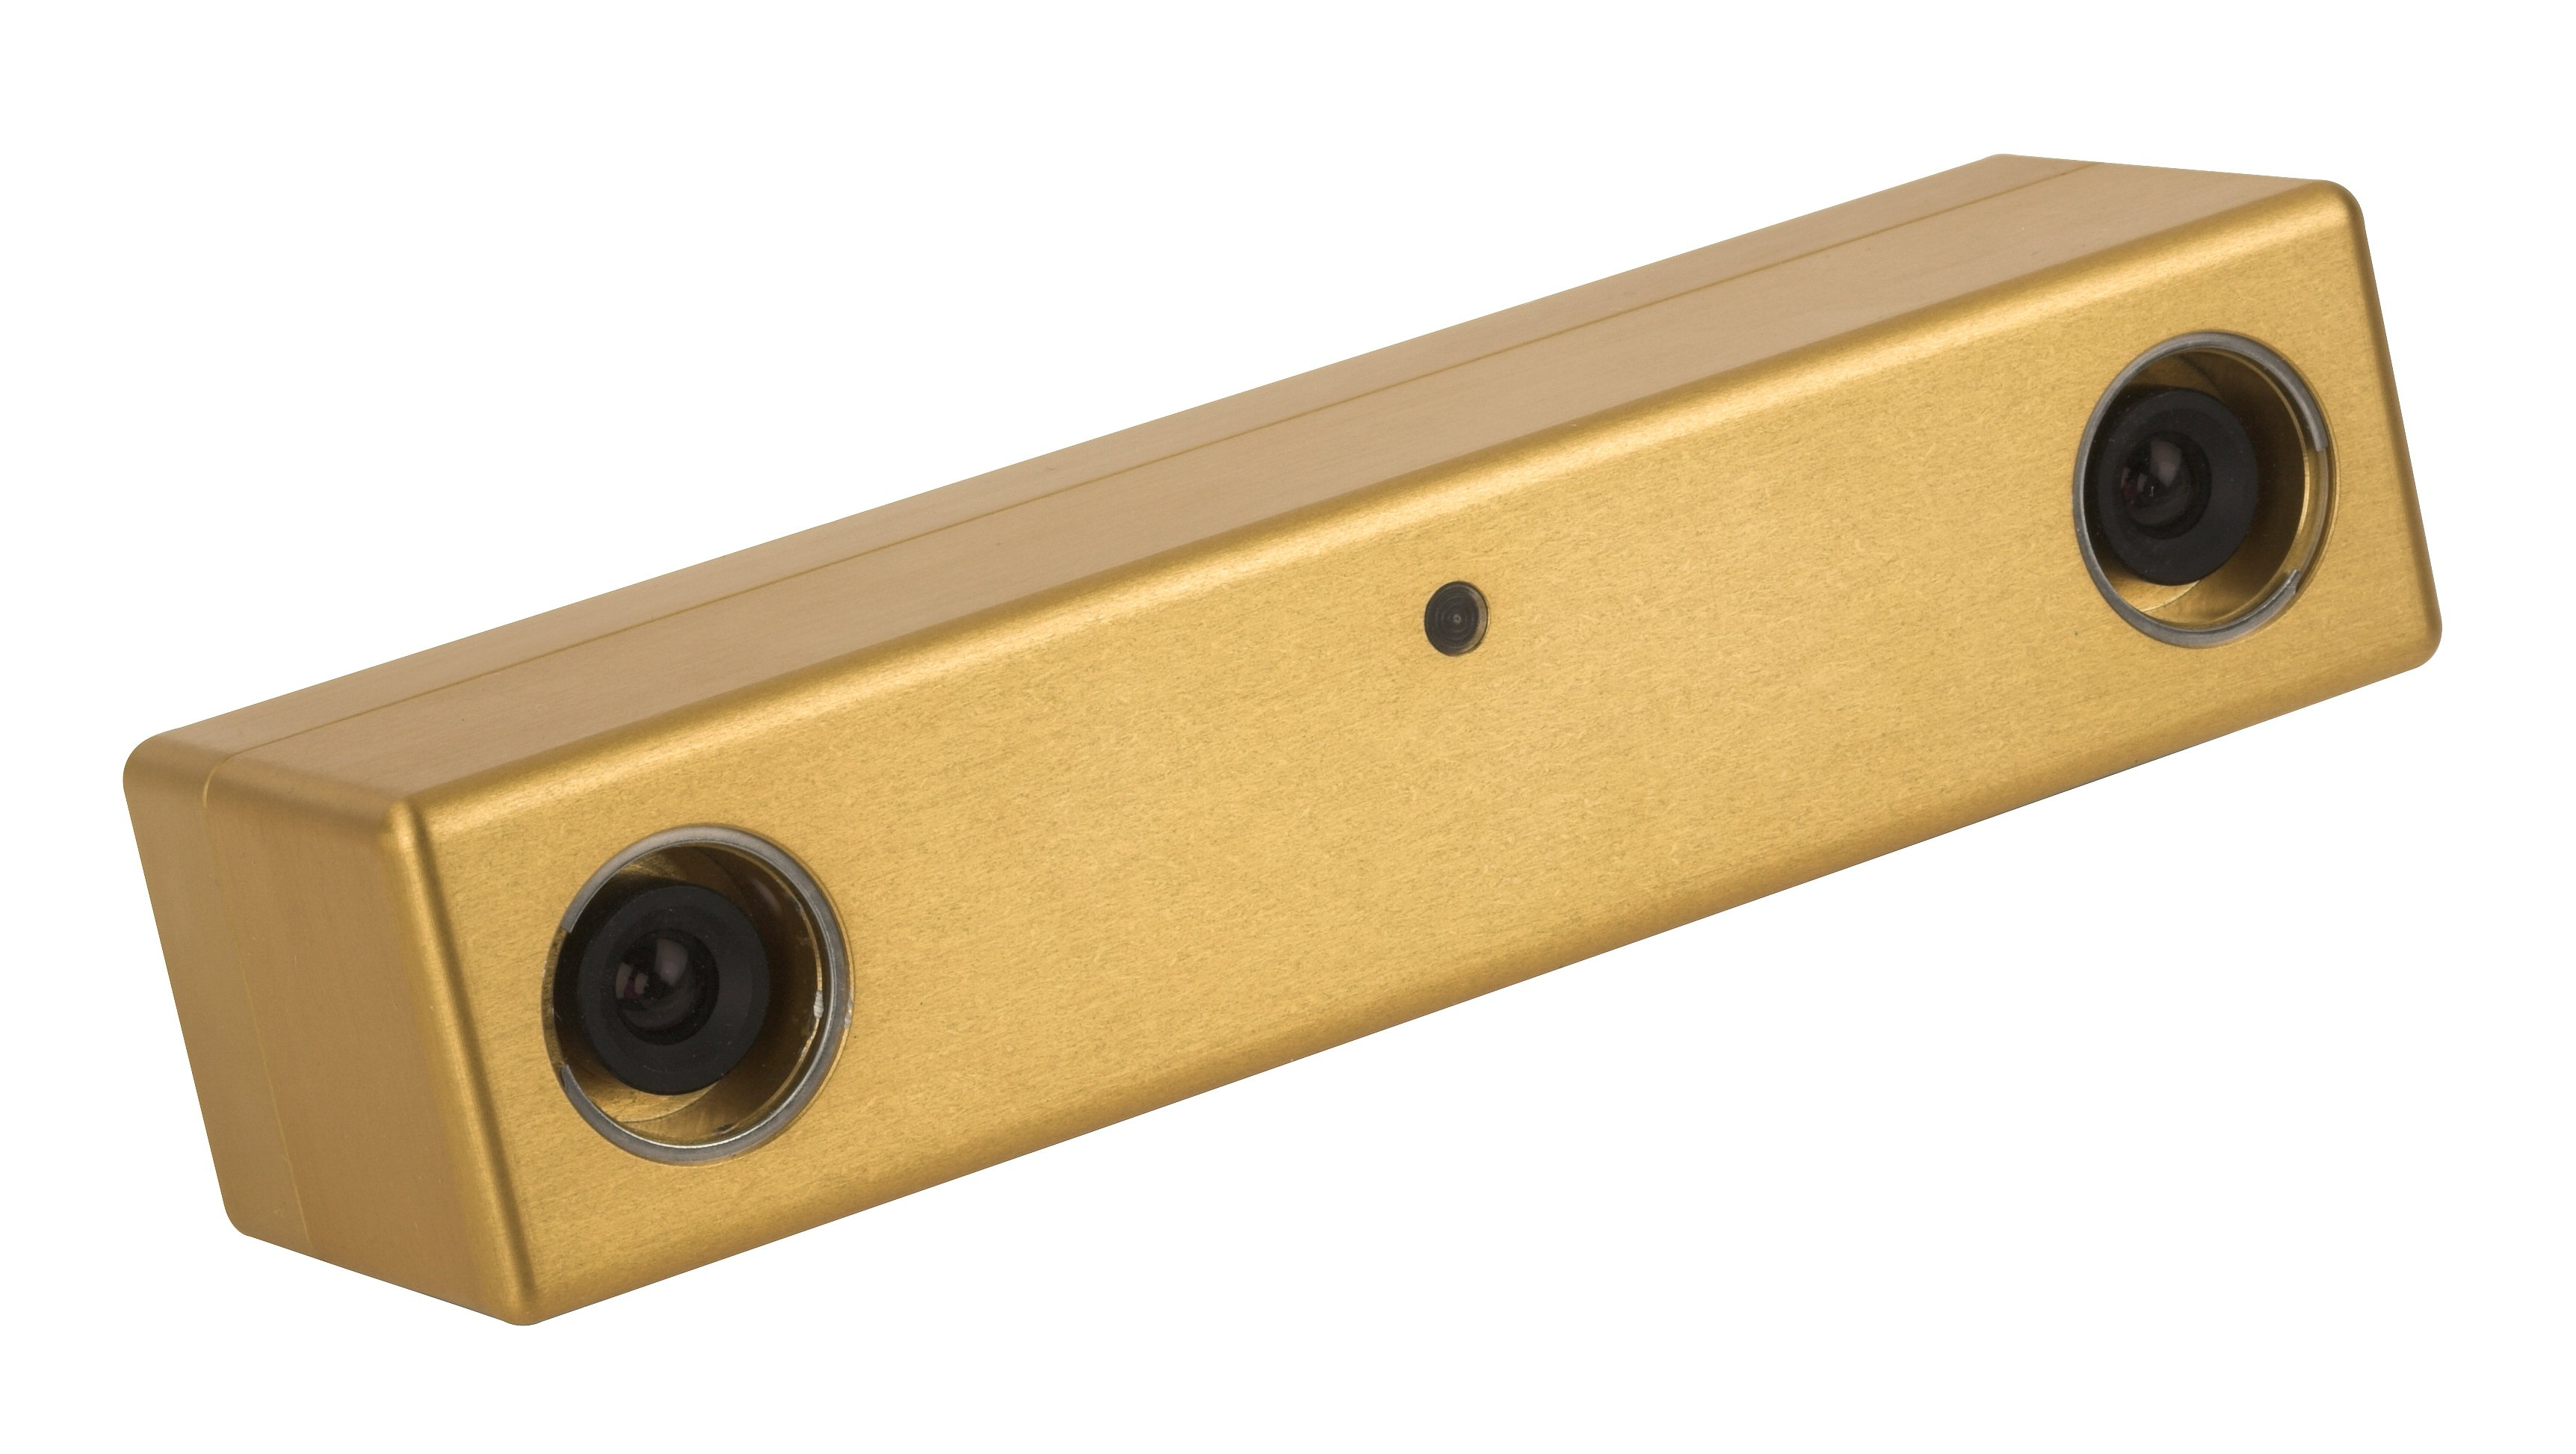
\includegraphics[width=3cm]{pictures/bumblebee.jpg}\label{subfig:bumblebee}}\vspace{4mm} \\
\subfloat[]{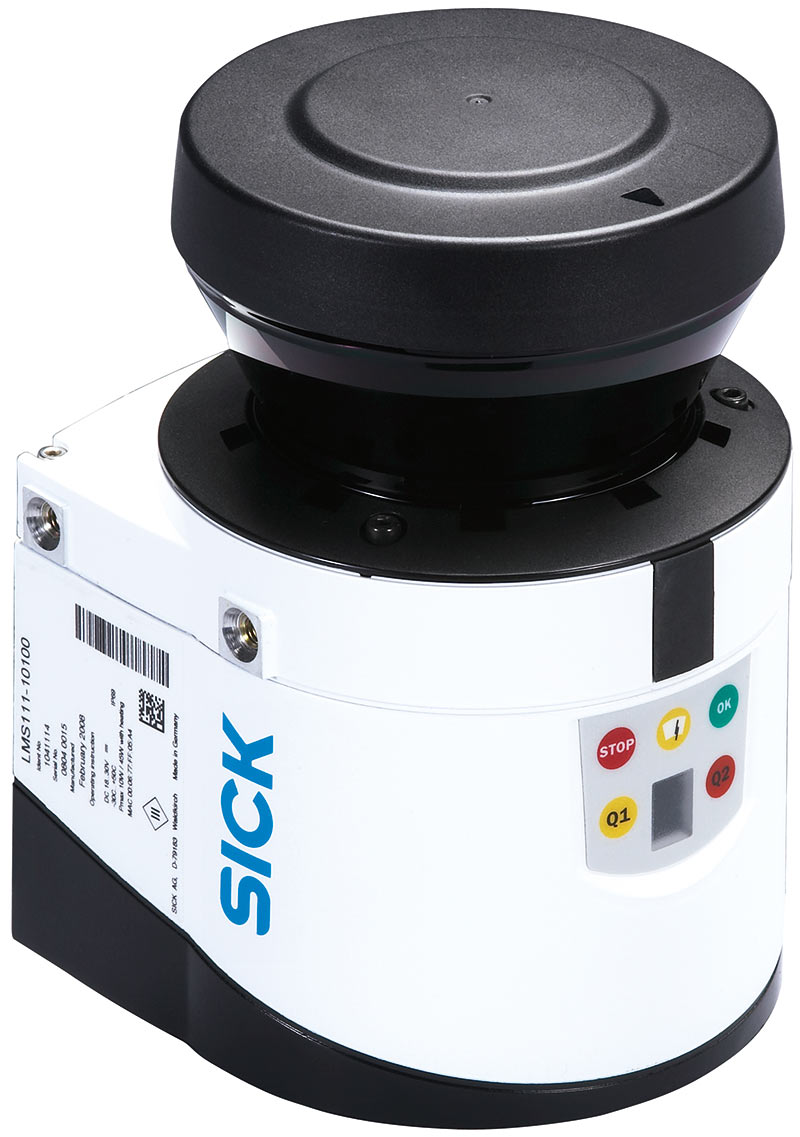
\includegraphics[width=2cm]{pictures/lms_2_0.jpg}\label{subfig:laser}} &
\multirow{-12}[3]{*}{\subfloat[]{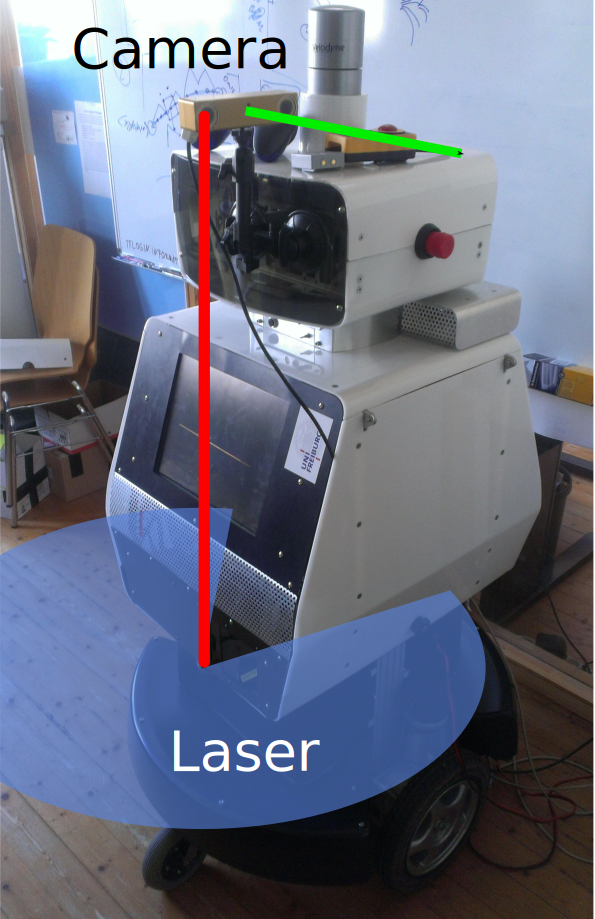
\includegraphics[width=4cm]{pictures/obelix.pdf}\label{subfig:obelix}}} \\
\end{tabular}
\caption{A Bumblebee stereo camera \subref{subfig:bumblebee} and a laser range finder \subref{subfig:laser} mounted on the Obelix robot on the same vertical axis \subref{subfig:obelix}.}
\end{figure}


\begin{figure}[p]%
\centering
\subfloat{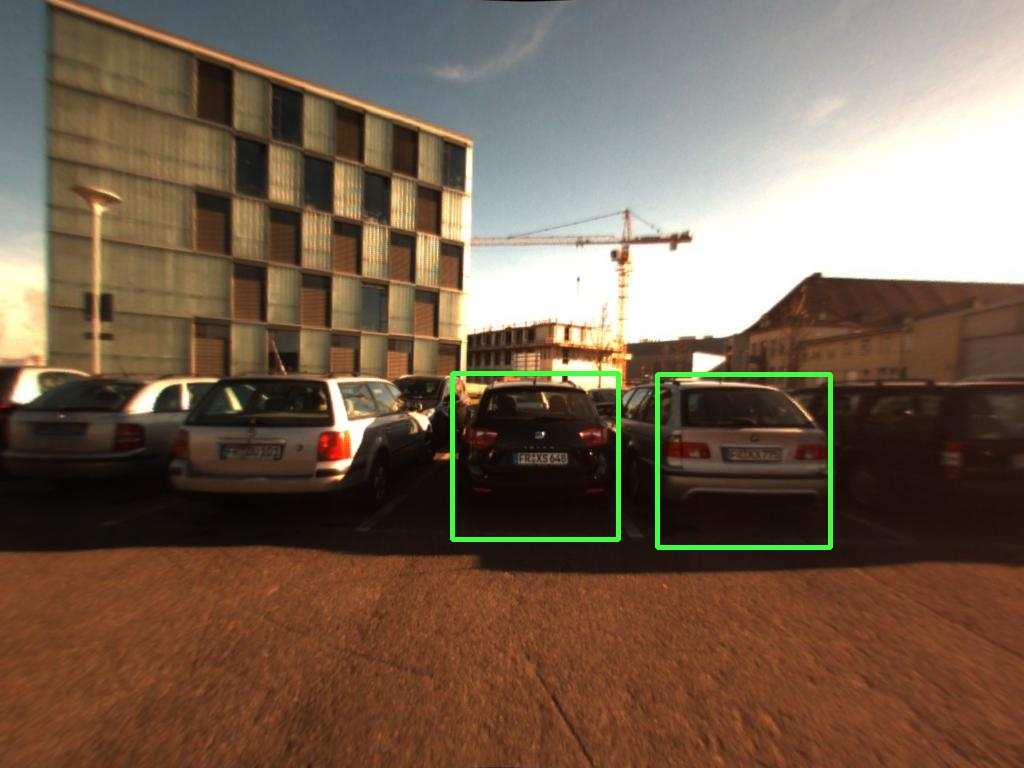
\includegraphics[width=0.3\textwidth]{pictures/det_1.jpg}}\hspace{2mm}
\subfloat{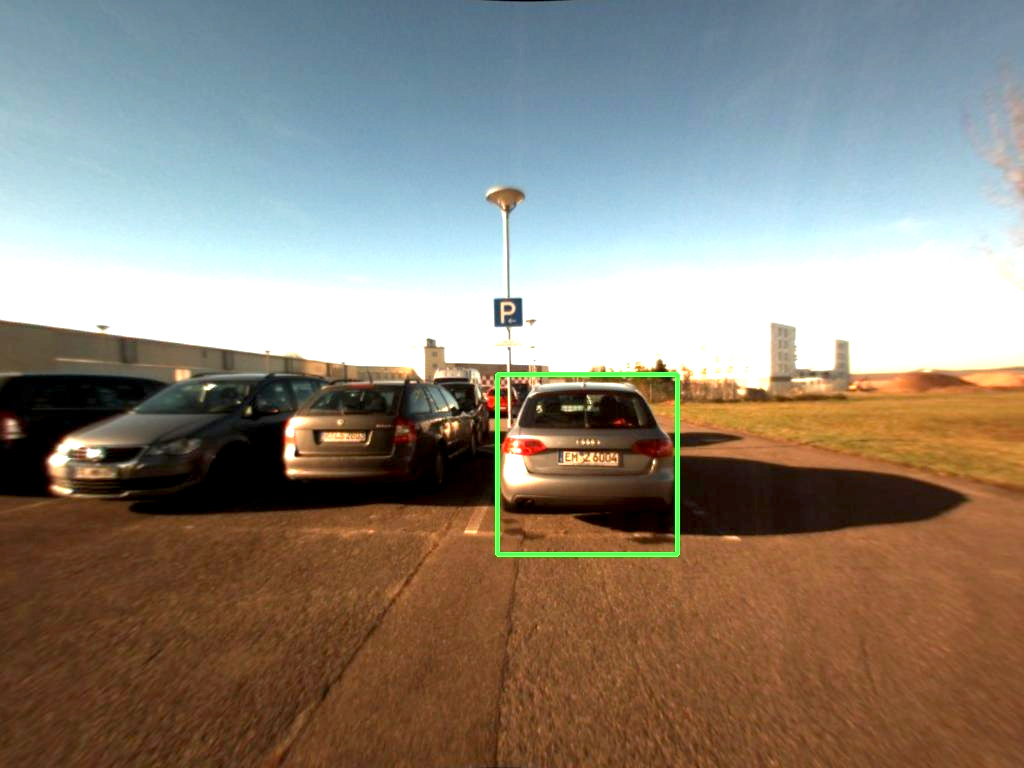
\includegraphics[width=0.3\textwidth]{pictures/det_2.jpg}}\hspace{2mm}
\subfloat{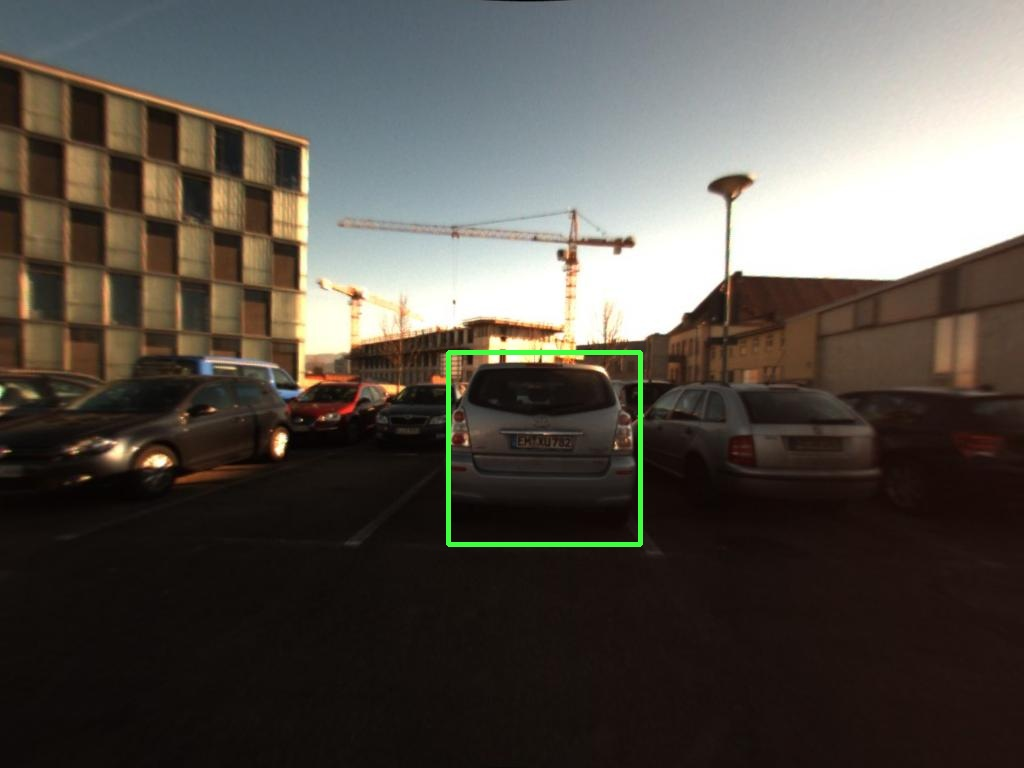
\includegraphics[width=0.3\textwidth]{pictures/det_3.jpg}}\\
\subfloat{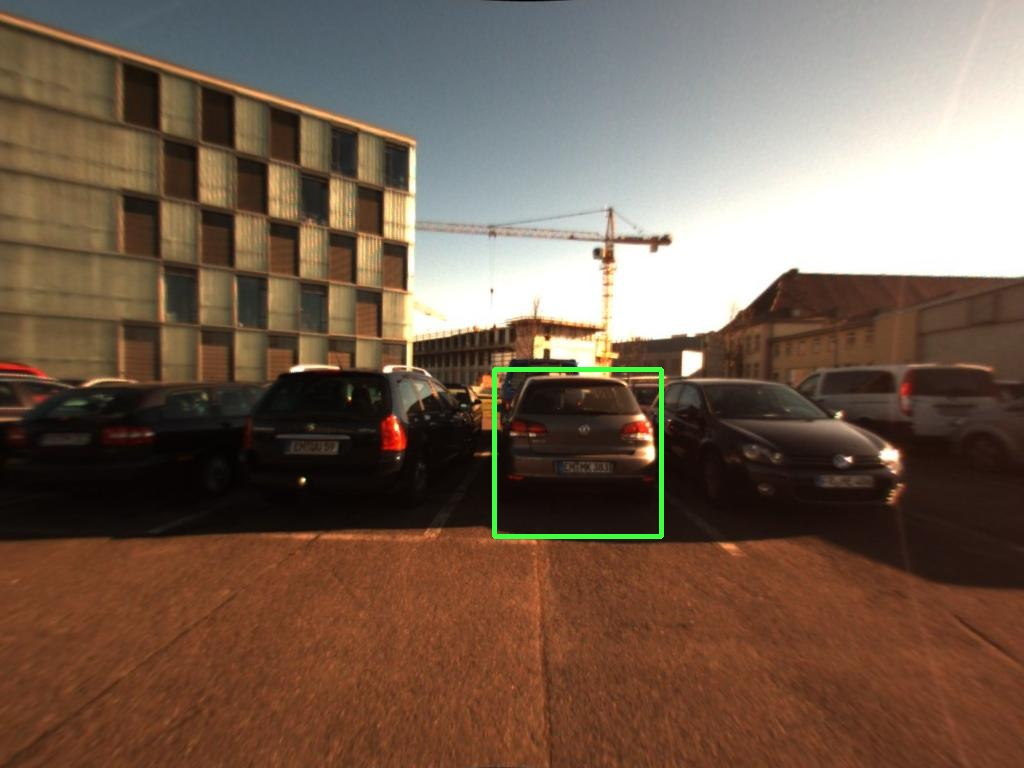
\includegraphics[width=0.3\textwidth]{pictures/det_4.jpg}}\hspace{2mm}
\subfloat{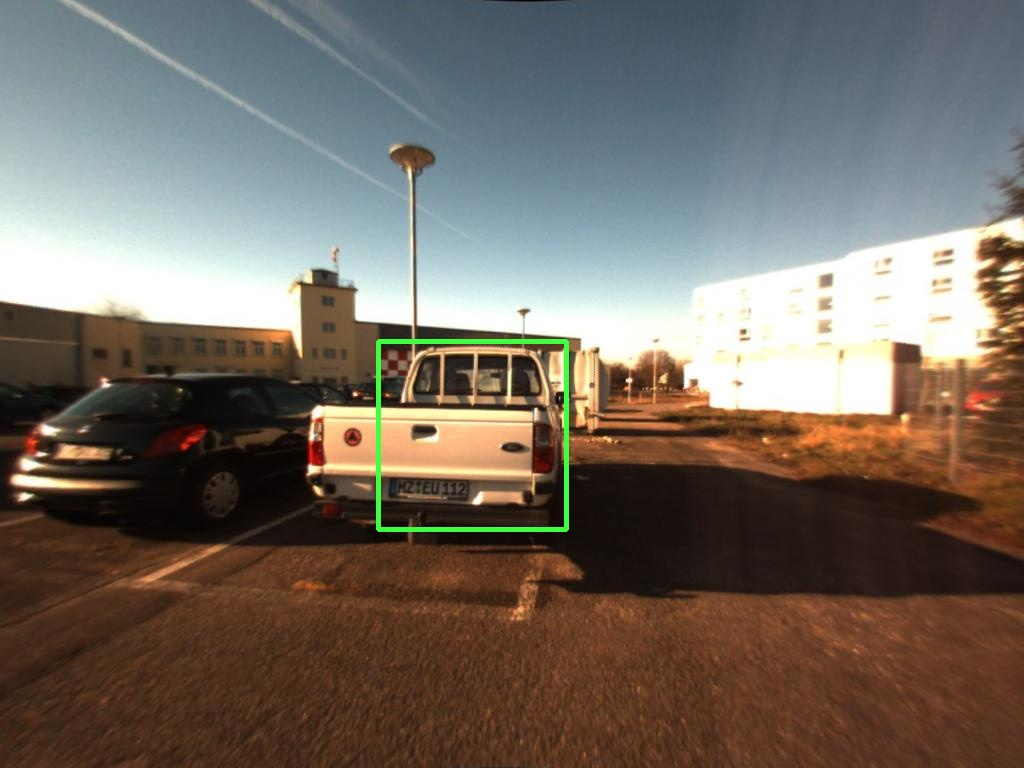
\includegraphics[width=0.3\textwidth]{pictures/det_5.jpg}}\hspace{2mm}
\subfloat{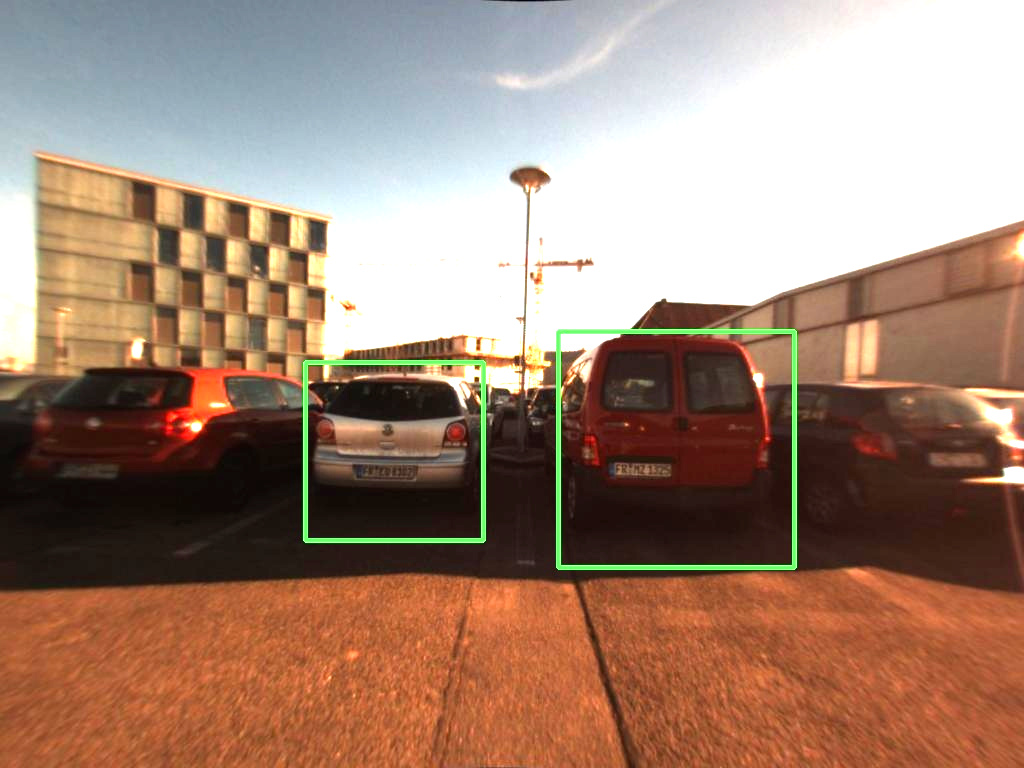
\includegraphics[width=0.3\textwidth]{pictures/det_6.jpg}}\\
\subfloat{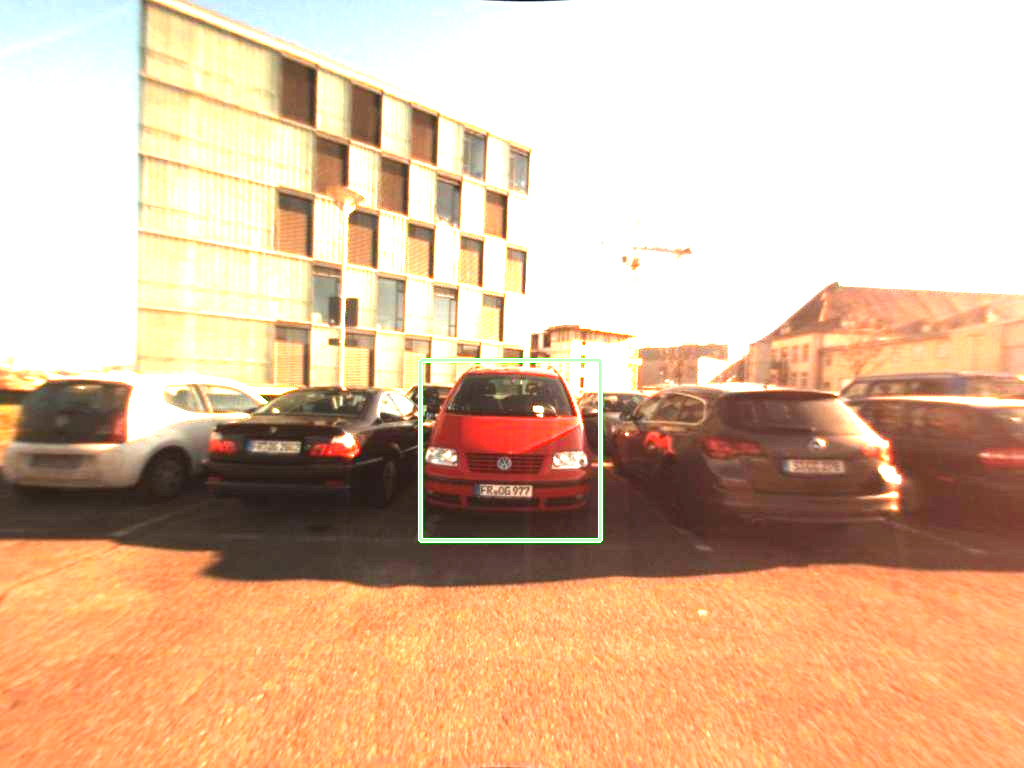
\includegraphics[width=0.3\textwidth]{pictures/det_7.jpg}}\hspace{2mm}
\subfloat{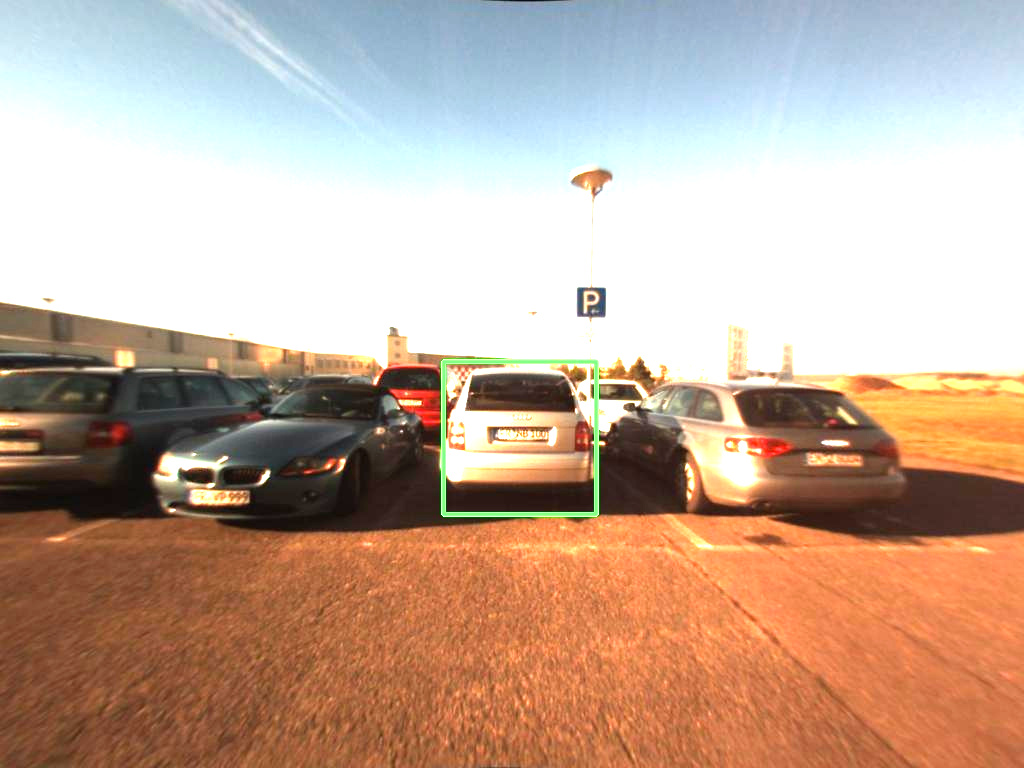
\includegraphics[width=0.3\textwidth]{pictures/det_8.jpg}}\hspace{2mm}
\subfloat{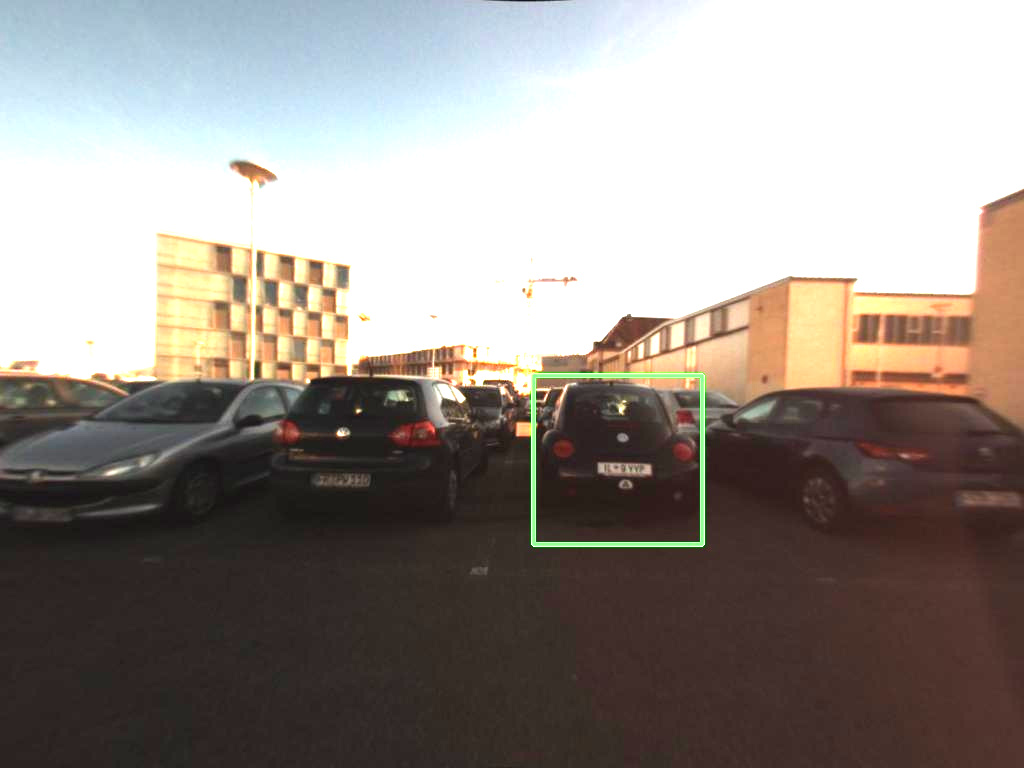
\includegraphics[width=0.3\textwidth]{pictures/det_9.jpg}}\\
\subfloat{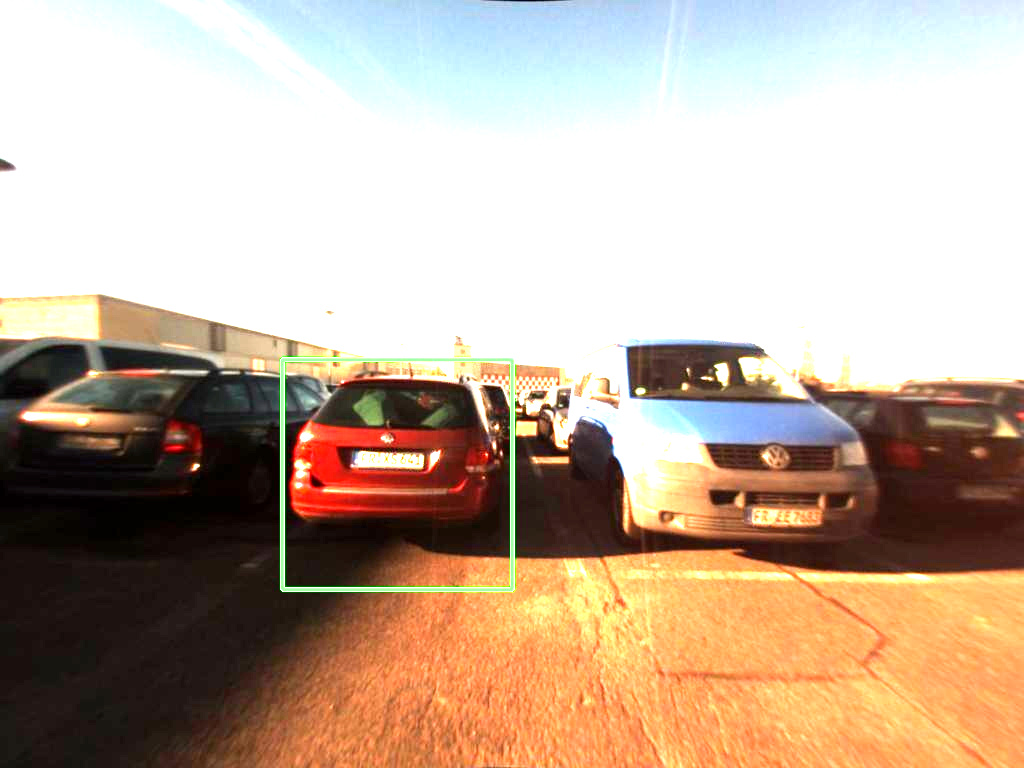
\includegraphics[width=0.3\textwidth]{pictures/det_10.jpg}}\hspace{2mm}
\subfloat{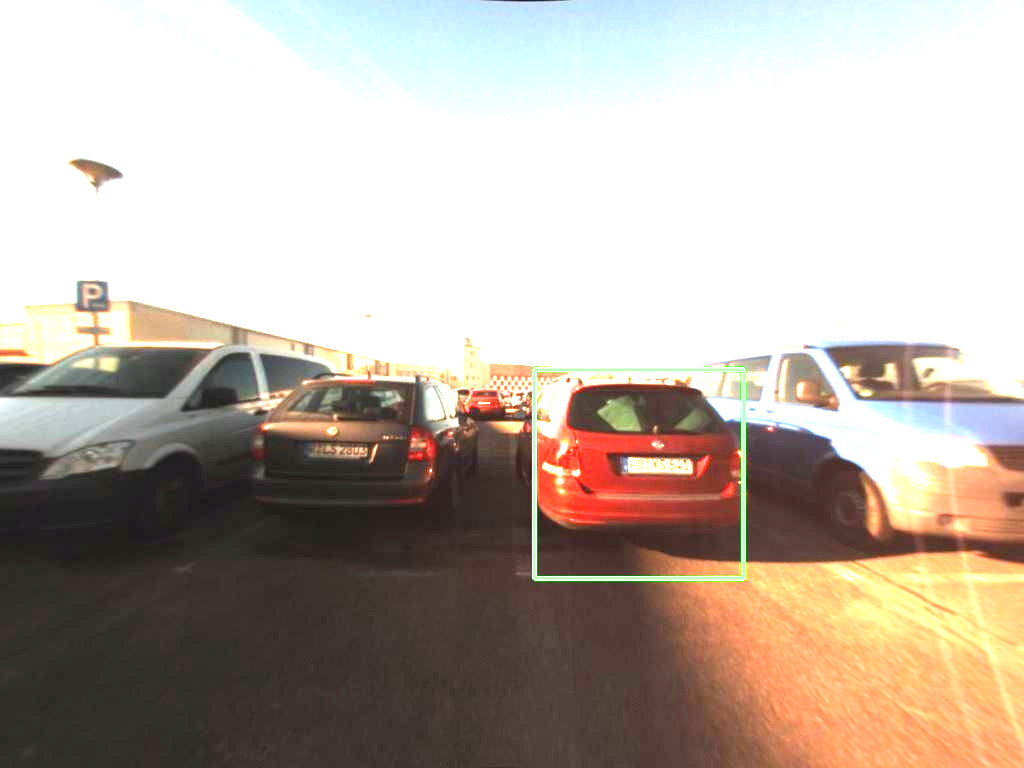
\includegraphics[width=0.3\textwidth]{pictures/det_11.jpg}}\hspace{2mm}
\subfloat{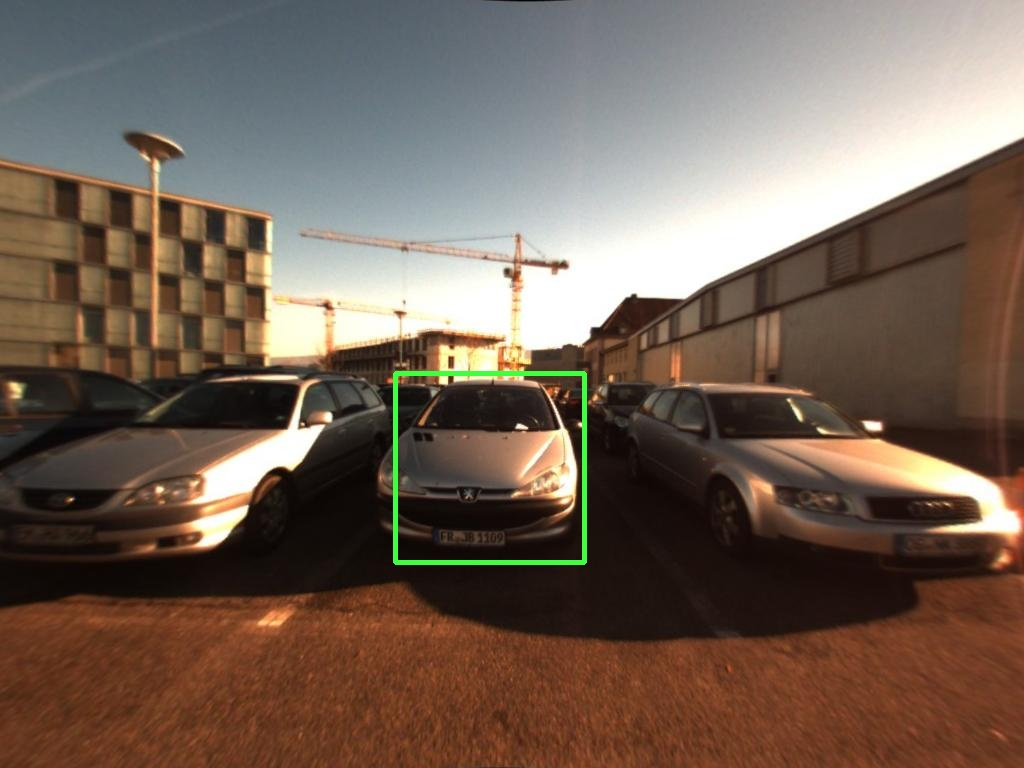
\includegraphics[width=0.3\textwidth]{pictures/det_12.jpg}}\\
\subfloat{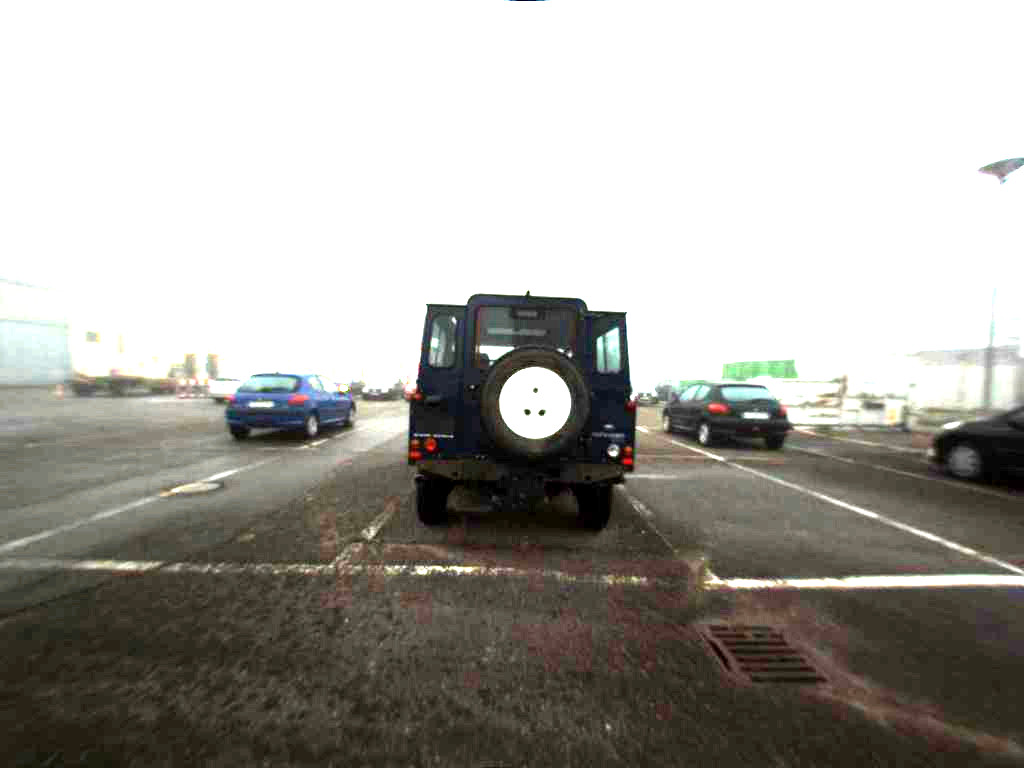
\includegraphics[width=0.3\textwidth]{pictures/undet_1.jpg}}\hspace{2mm}
\subfloat{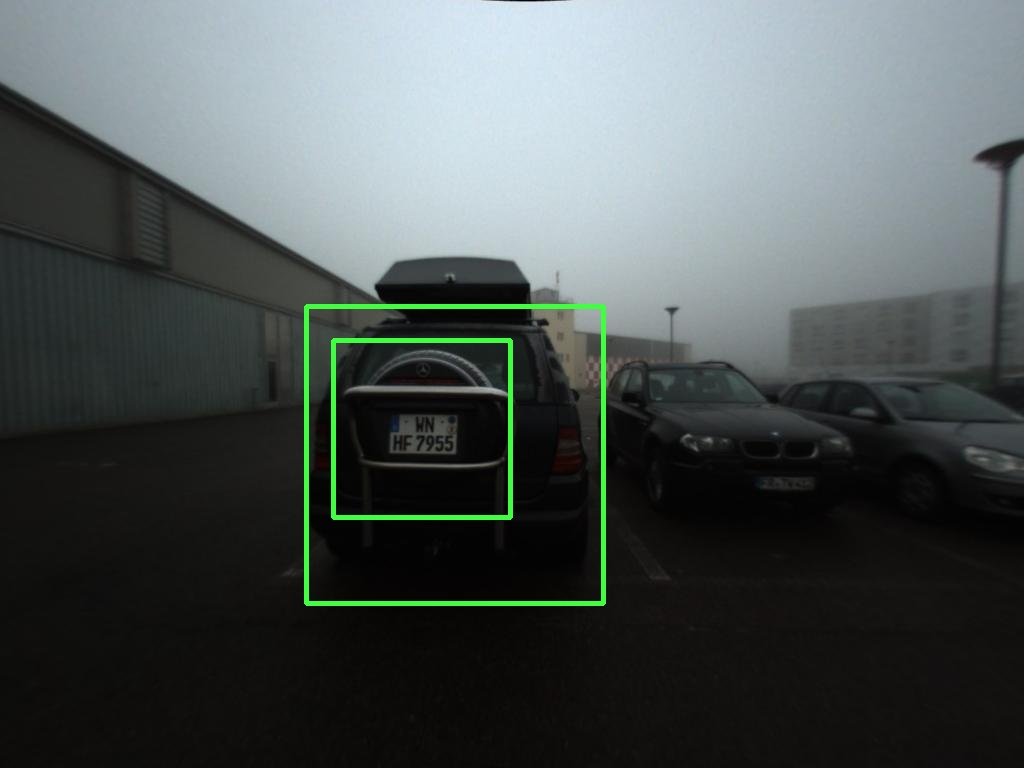
\includegraphics[width=0.3\textwidth]{pictures/undet_2.jpg}}\hspace{2mm}
\subfloat{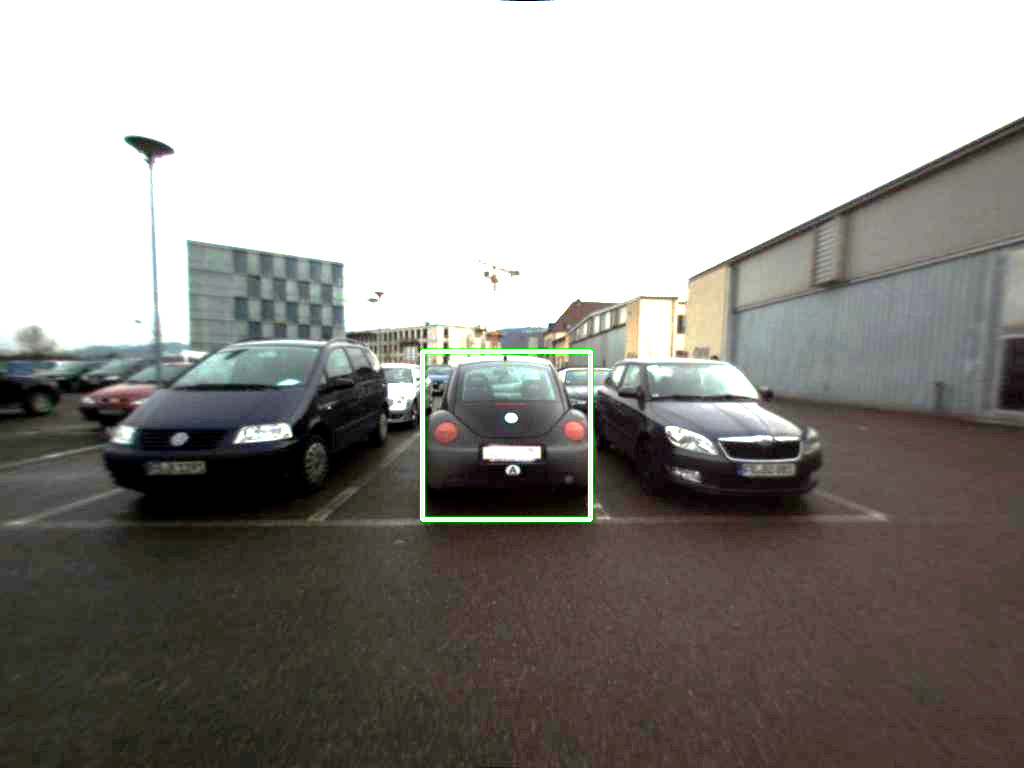
\includegraphics[width=0.3\textwidth]{pictures/det_14.jpg}}\\
\caption{Examples of detections of different cars under different light conditions.}
\label{fig:detection_examples}
\end{figure}

% section visual_car_detection (end)

\section{Parking Lot Modeling}
\label{sec:parking_lots_modeling}

\begin{figure}[p]%
\centering
\subfloat[Aerial view.]{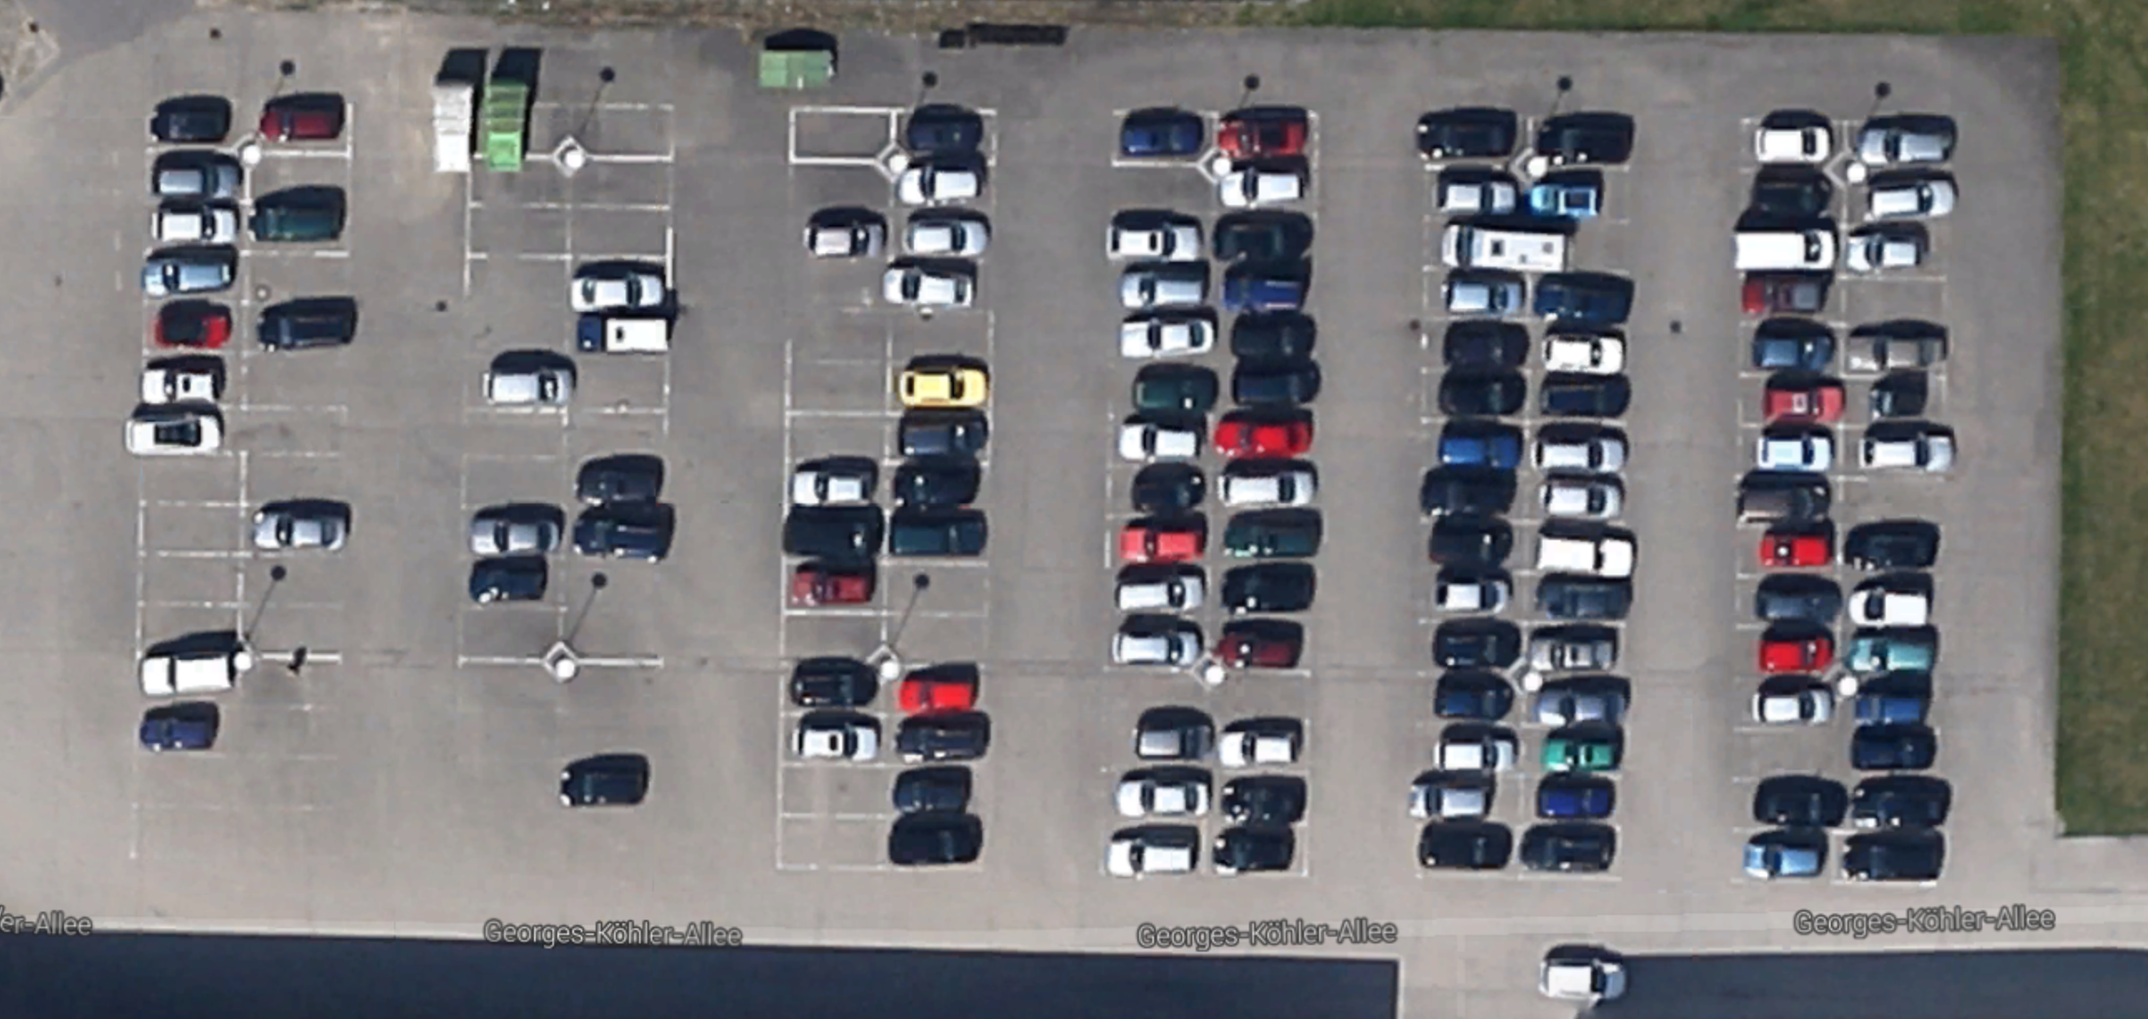
\includegraphics[width=0.6\textwidth]{pictures/google_map.pdf}\label{subfig:aerial}} \\
\subfloat[Car detections over the map built with the laser-based SLAM procedure.]{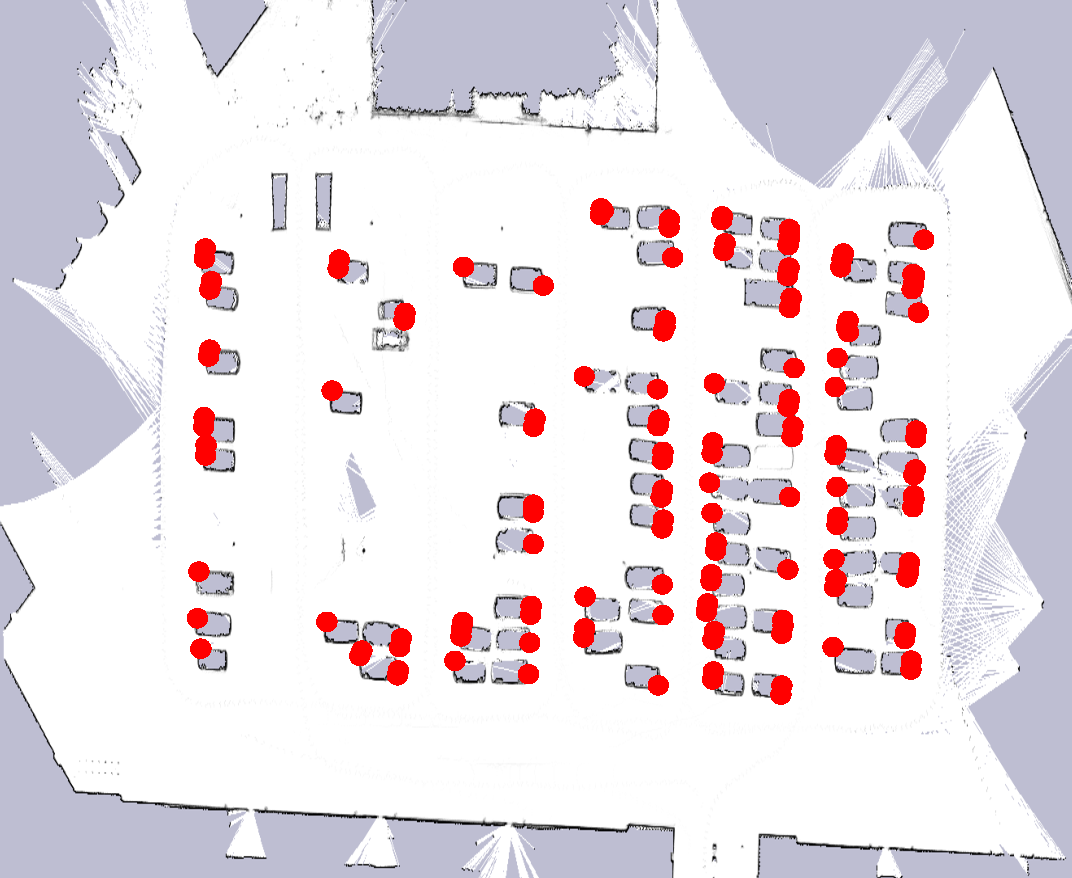
\includegraphics[width=0.6\textwidth]{pictures/laser_fusion.pdf}\label{subfig:slam_detections}} \\
\subfloat[Occupancy grid map acquired as described in Section~\ref{sub:occupancy_grids}.]{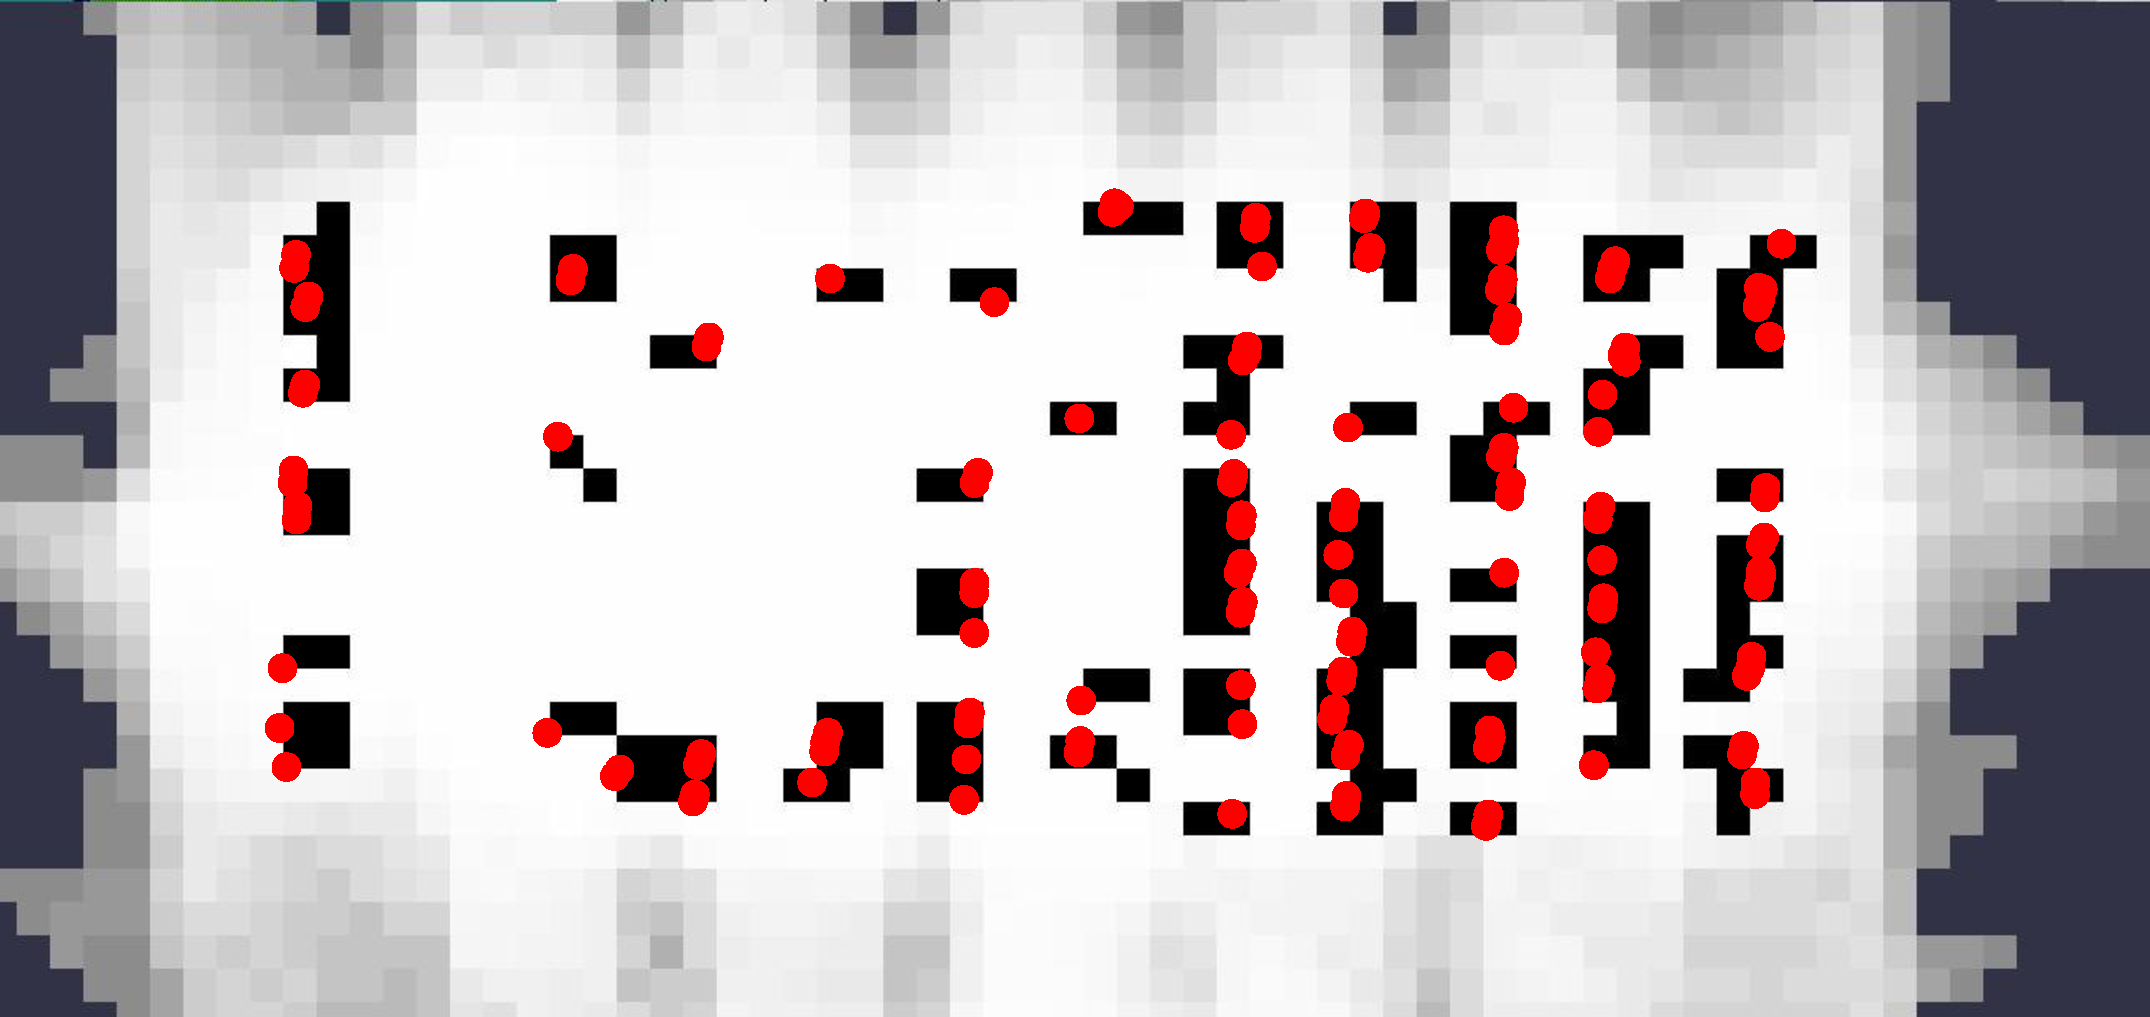
\includegraphics[width=0.6\textwidth]{pictures/occupancy_cars.pdf}\label{subfig:occ_maps_detections}} \\
\subfloat[Cars positions mapped to pre-defined parking lot positions.]{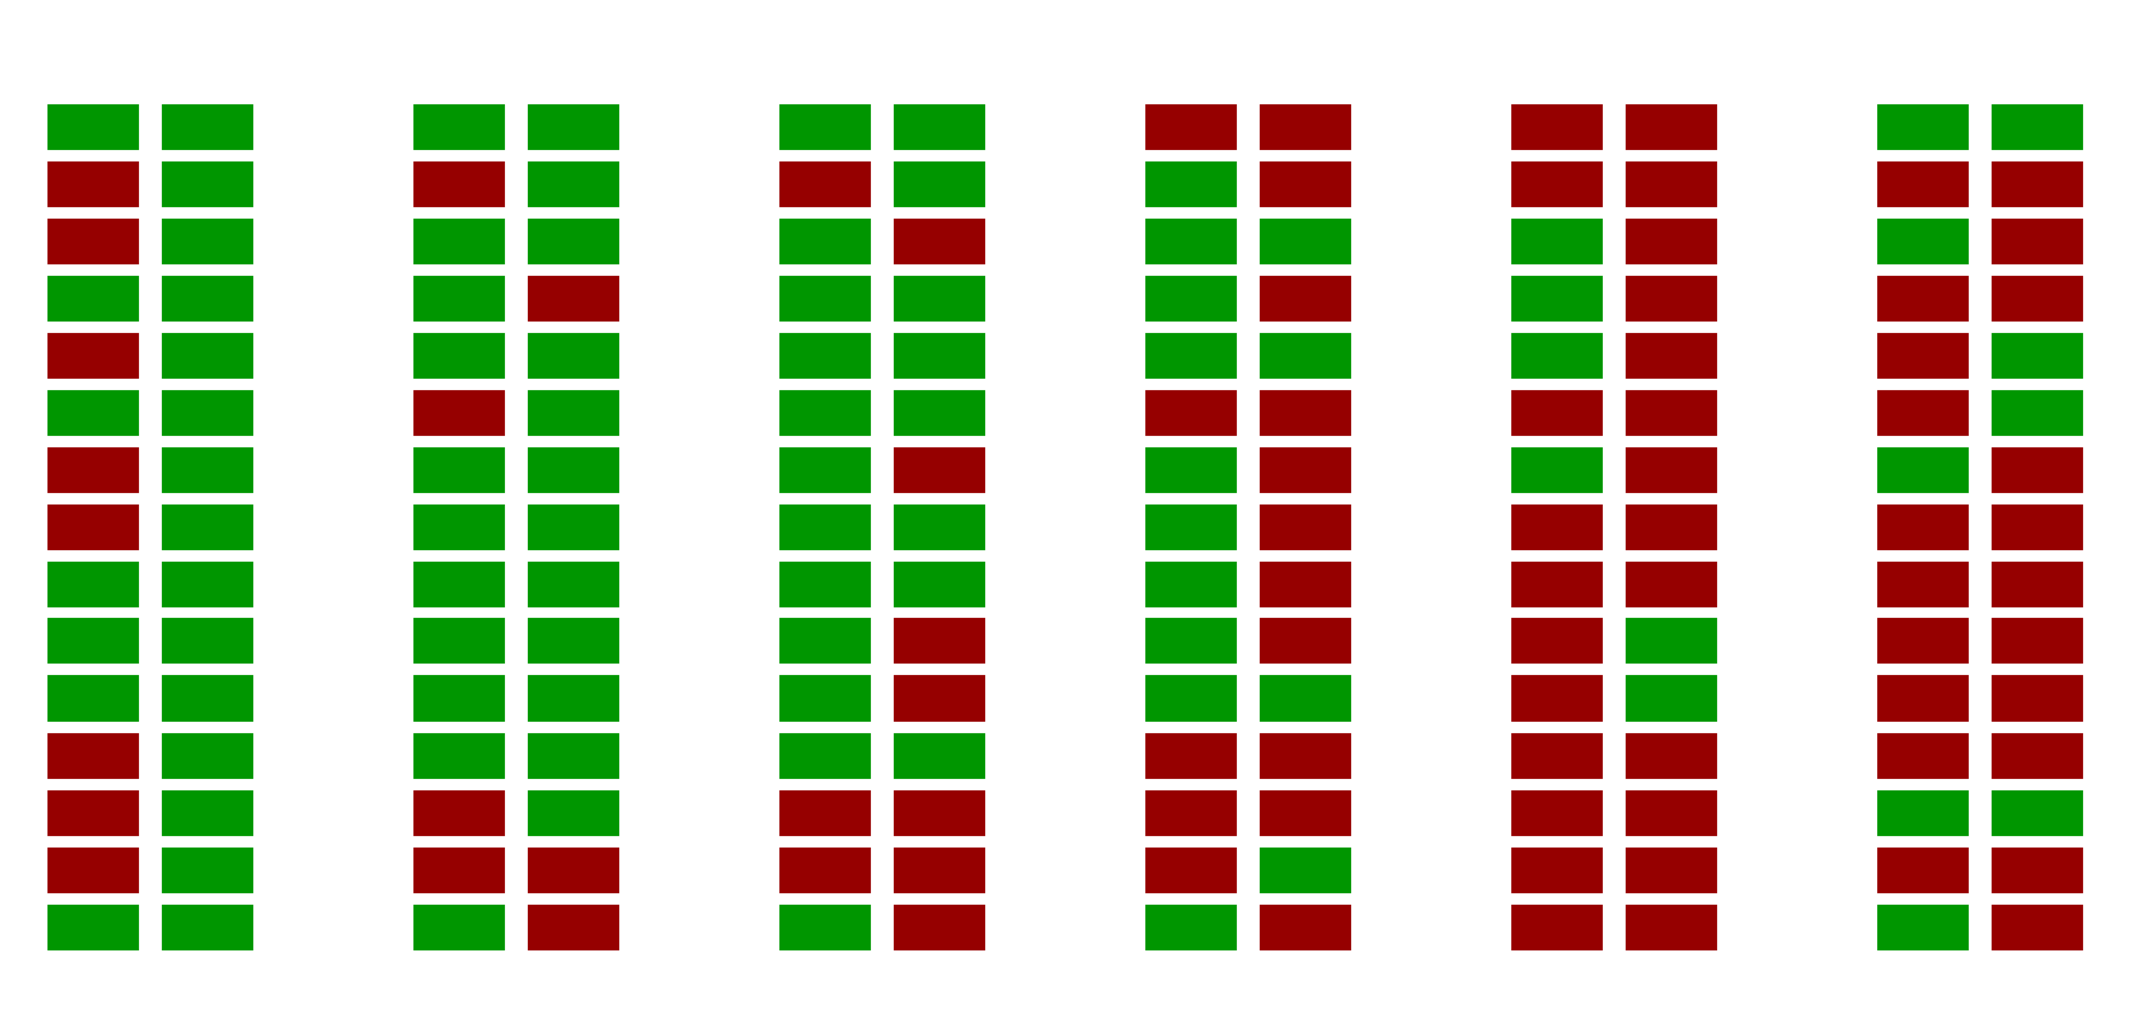
\includegraphics[width=0.6\textwidth]{pictures/parking_lots_detections.pdf}\label{subfig:pre_defined}}
\caption{Representations of the campus parking lot at the university of Freiburg. \\ Images \subref{subfig:slam_detections}, \subref{subfig:occ_maps_detections},~\subref{subfig:pre_defined}  represent the same occupancy state of the parking lot.}
\label{fig:different_mappings}
\end{figure}

The occupancy data is based on the 2D data obtained either from the stereo
cameras (Figure~\ref{subfig:bumblebee}) or from laser range finder, mounted on
the robot (Figure~\ref{subfig:laser}). As can be seen in the figure, the
stereo camera is mounted on the same z-axis with the laser range finder. We
search for the endpoints that represent the cars as described in the section
\nameref{sec:perception} of chapter \nameref{cha:our_approach}.

Figure~\ref{fig:depth_from_disparity} shows that the depth information
computed from the disparity image between two stereo images lacks precision
and has a significant amount of noise. Not only this noise is caused by the
method of depth estimation and errors in point association, but it also
suffers from the windows present in almost any car. The windows are
transparent which results in wrong depth measurements present in the detected
regions of interest.

To avoid the high noise from the stereo camera, we use the depth measurements
from a laser range finder. Each laser measurement has high precision in
measuring the distance. Because of its mounting position on the human knee
level, it also does not suffer from the partial transparency of the cars as
individual laser beams never encounter the cars' windows.

We present occupancy data aggregated to the occupancy grids as well as into
pre-defined parking lot positions. The illustration of differences in the maps
representations can be seen in Figure~\ref{fig:different_mappings}. The figure
shows car detected  cars positions as red dots. We produce these detections
fusing the laser range finder measurements with the visual detections as
described in Chapter~\ref{ssub:laser_range_finder}.

There are two distinct ways in which we model the parking lots: occupancy grid
maps and pre-defined parking lots positions.

As can be seen from the Figure~\ref{subfig:occ_maps_detections} the occupancy
grid based representation lacks precision. The main problem are the
discretization errors. It is a common situation when the detections on
different sides of the same car fall into different grid cells, causing
erroneous map representation. Another problem of the occupancy grid based
approach is an imperfect approximation of the car orientation. We argue, that
using the observation model, as seen in Figure~\ref{fig:maptest}, yields the
orientation of the detected car to be influenced by the angle from which it is
observed.

\begin{figure}[t]
    \begin{center}
        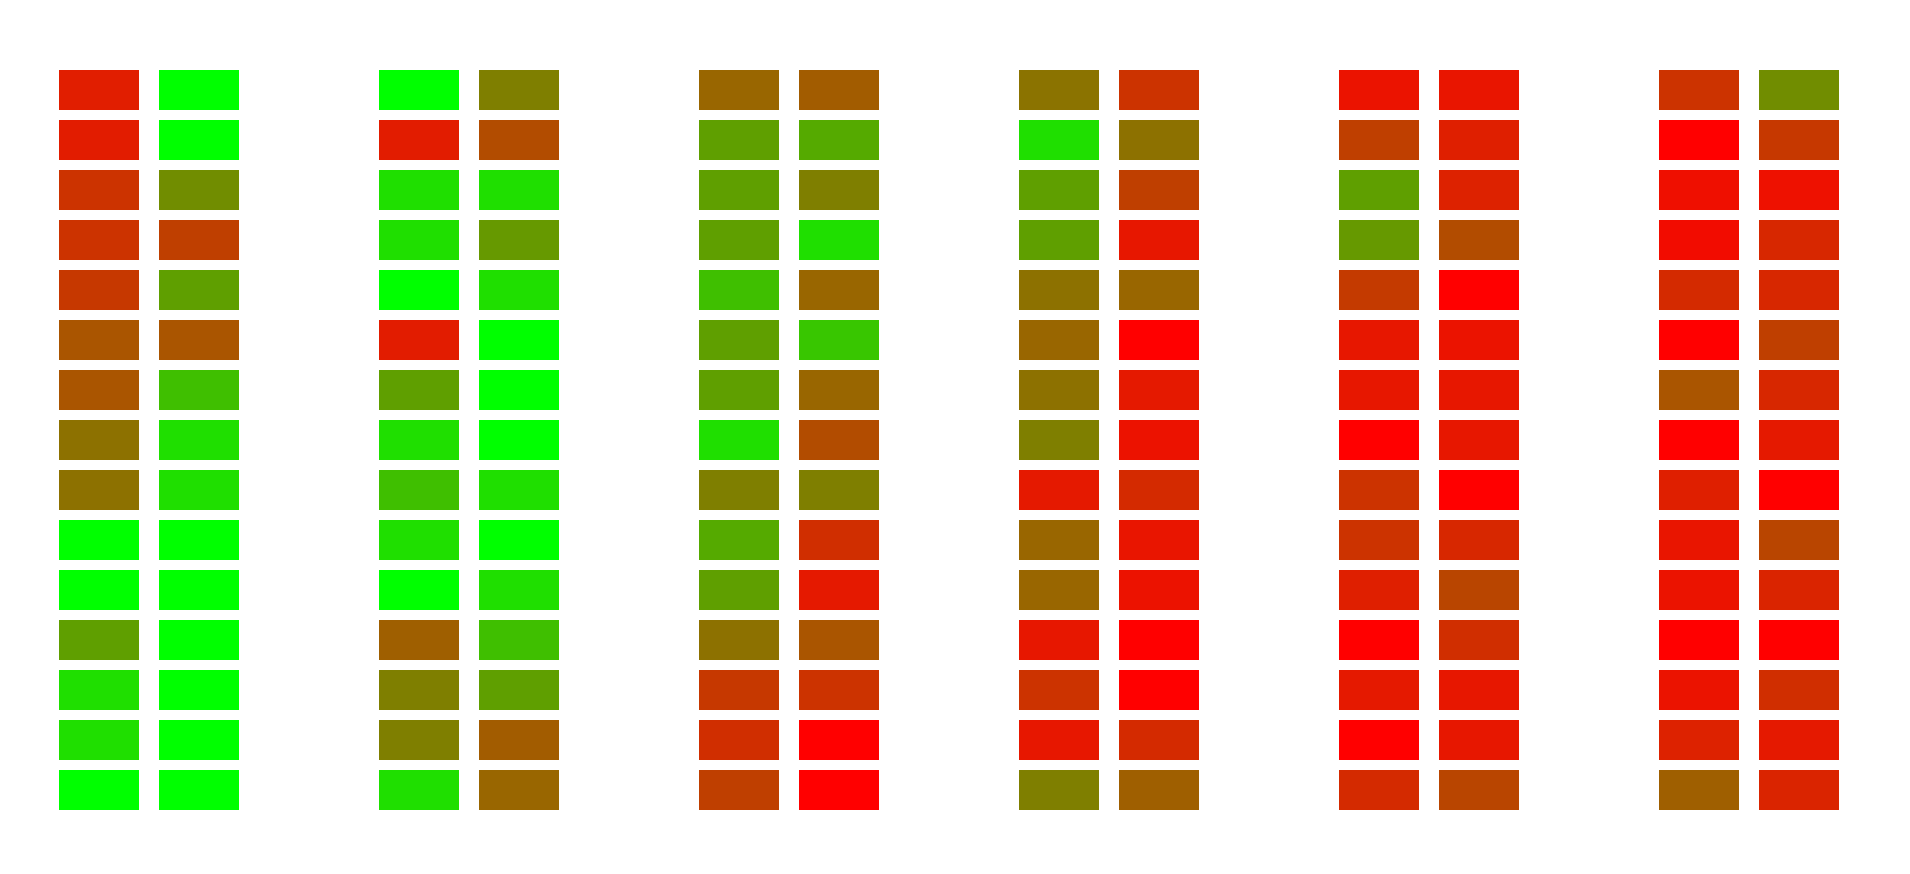
\includegraphics[width=0.6\textwidth]{pictures/parking_lots.png}
    \end{center}
    \caption{Occupancy probability accumulated during a sequence of observations shown in color. The greener the parking lot is --- the bigger the probability for it to be free.}
    \label{fig:occupancy_accumulated}
\end{figure}


\begin{figure}[p]%
\centering
\subfloat{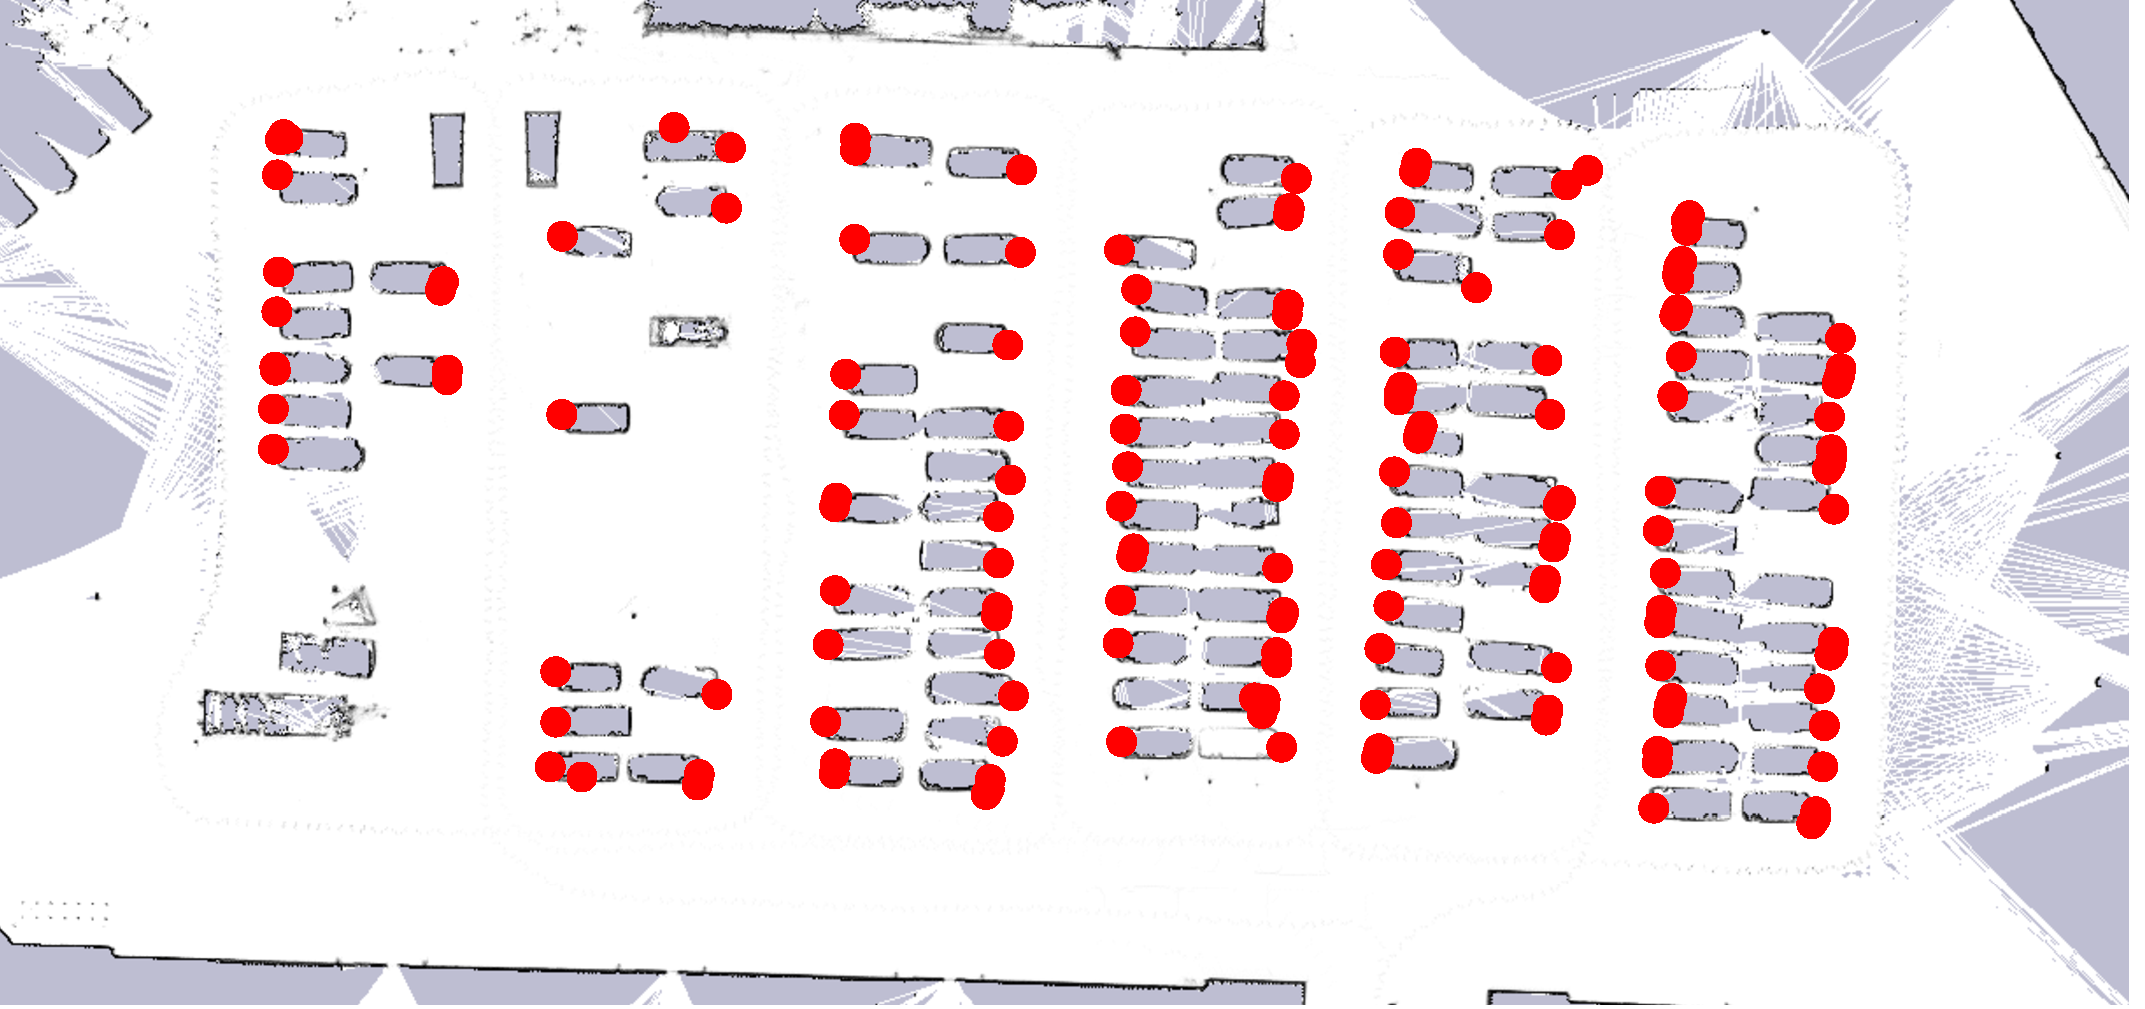
\includegraphics[width=0.47\textwidth]{pictures/laser_fusion_13_12.pdf}}\hspace{2mm}
\subfloat{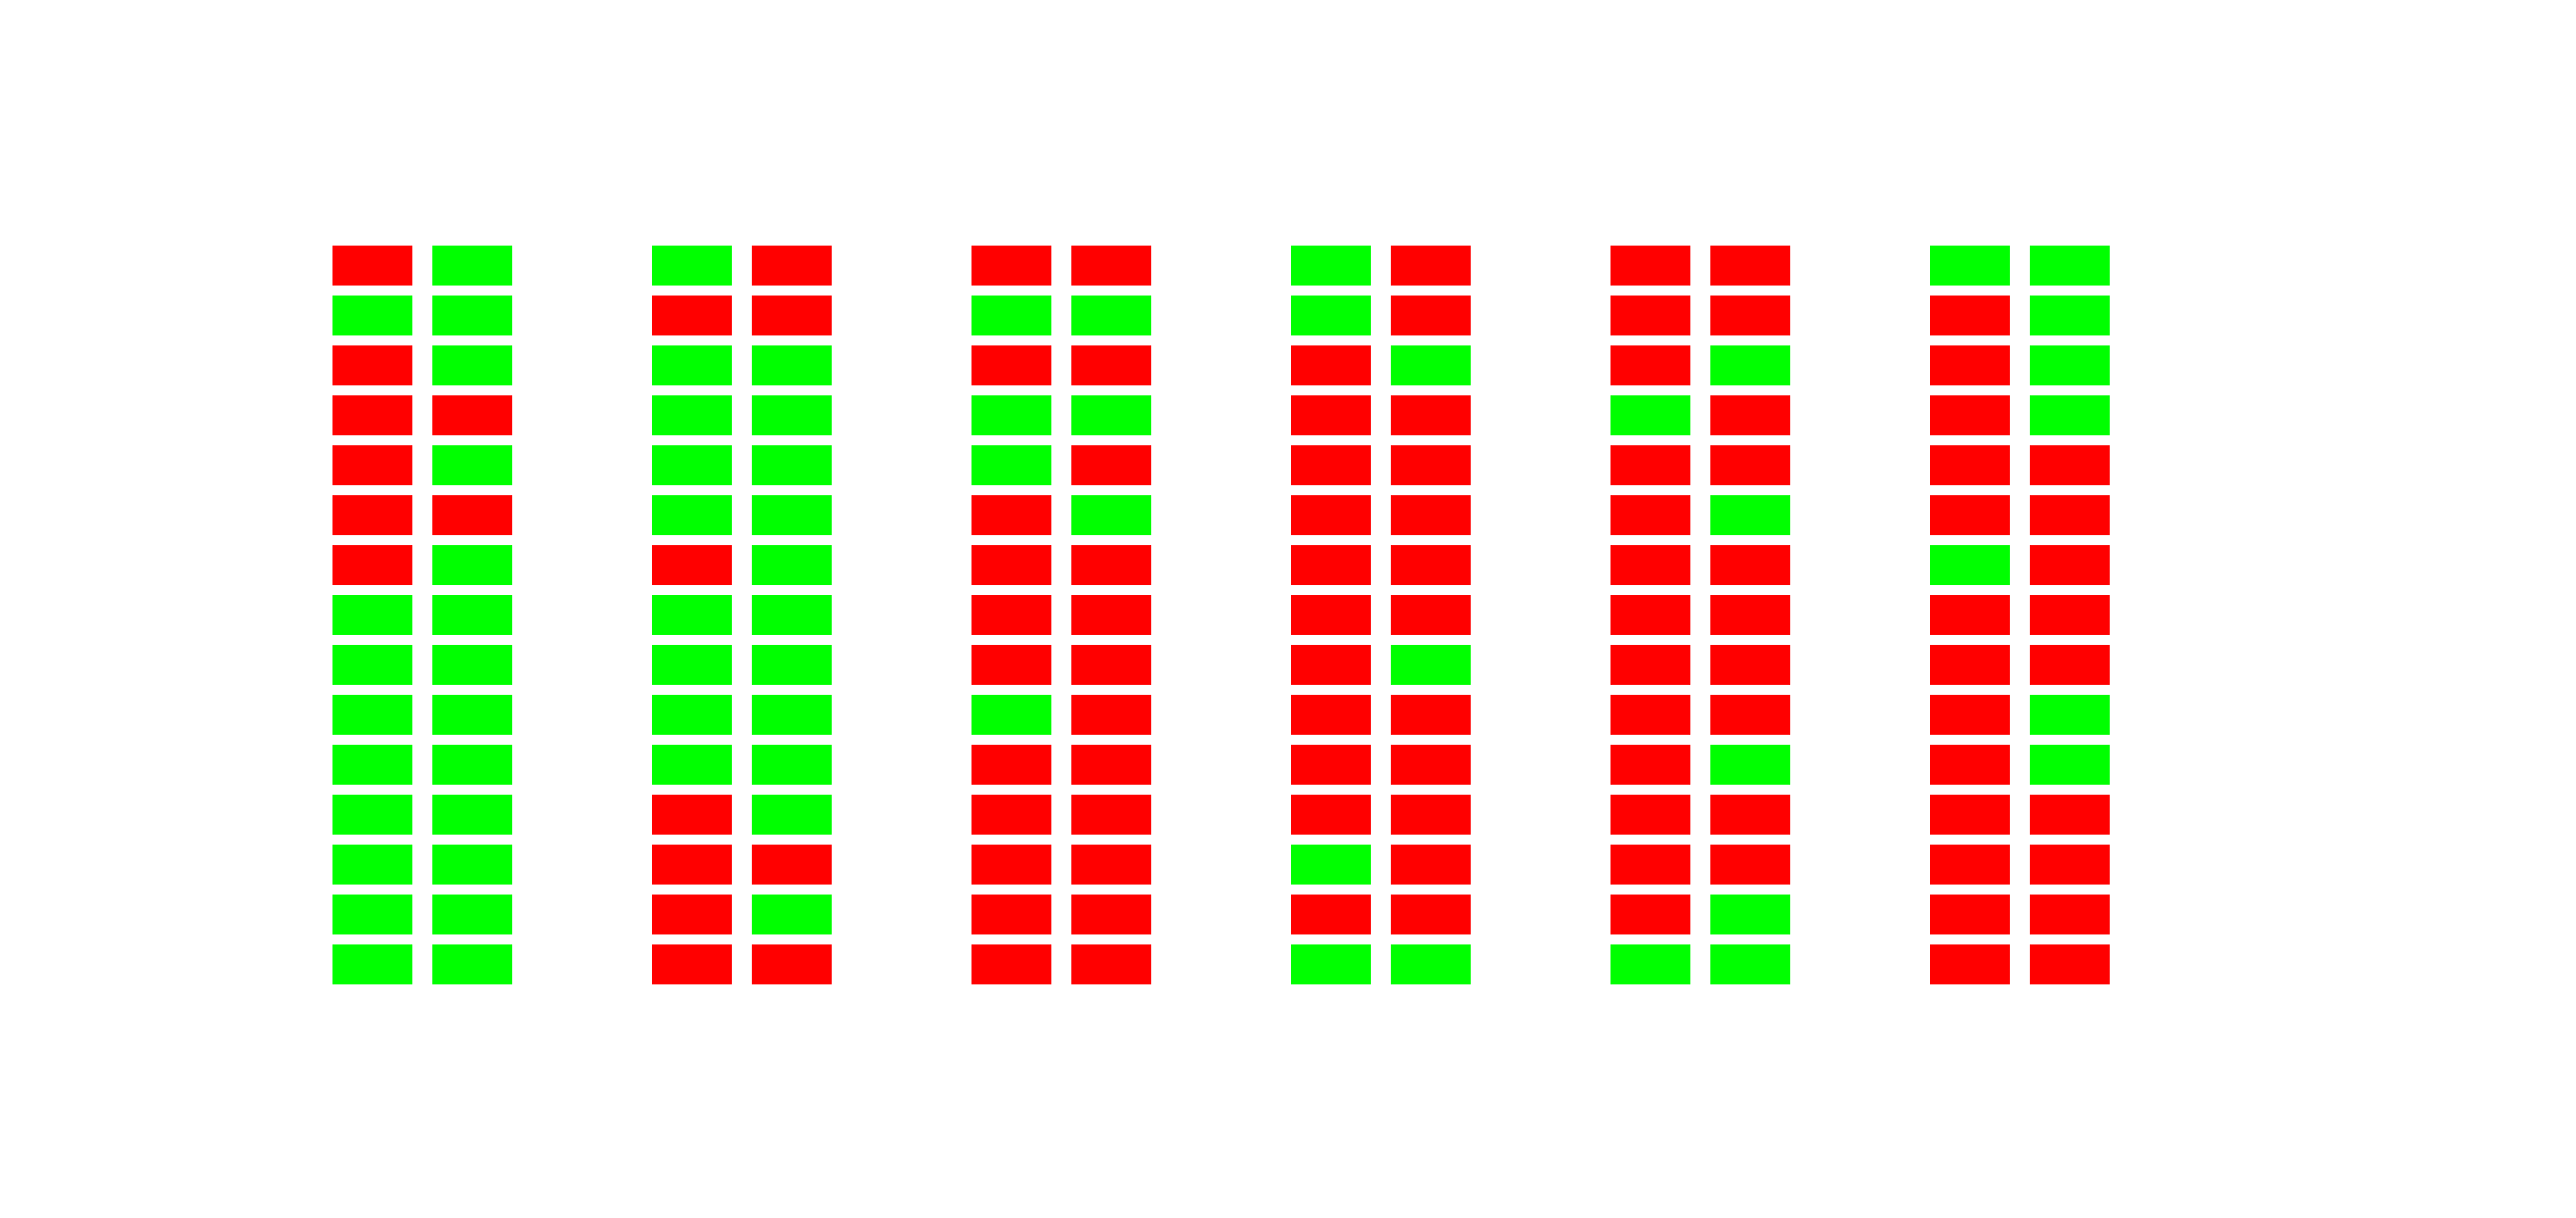
\includegraphics[width=0.47\textwidth]{pictures/parking_lots_13_12.png}}\\
\subfloat{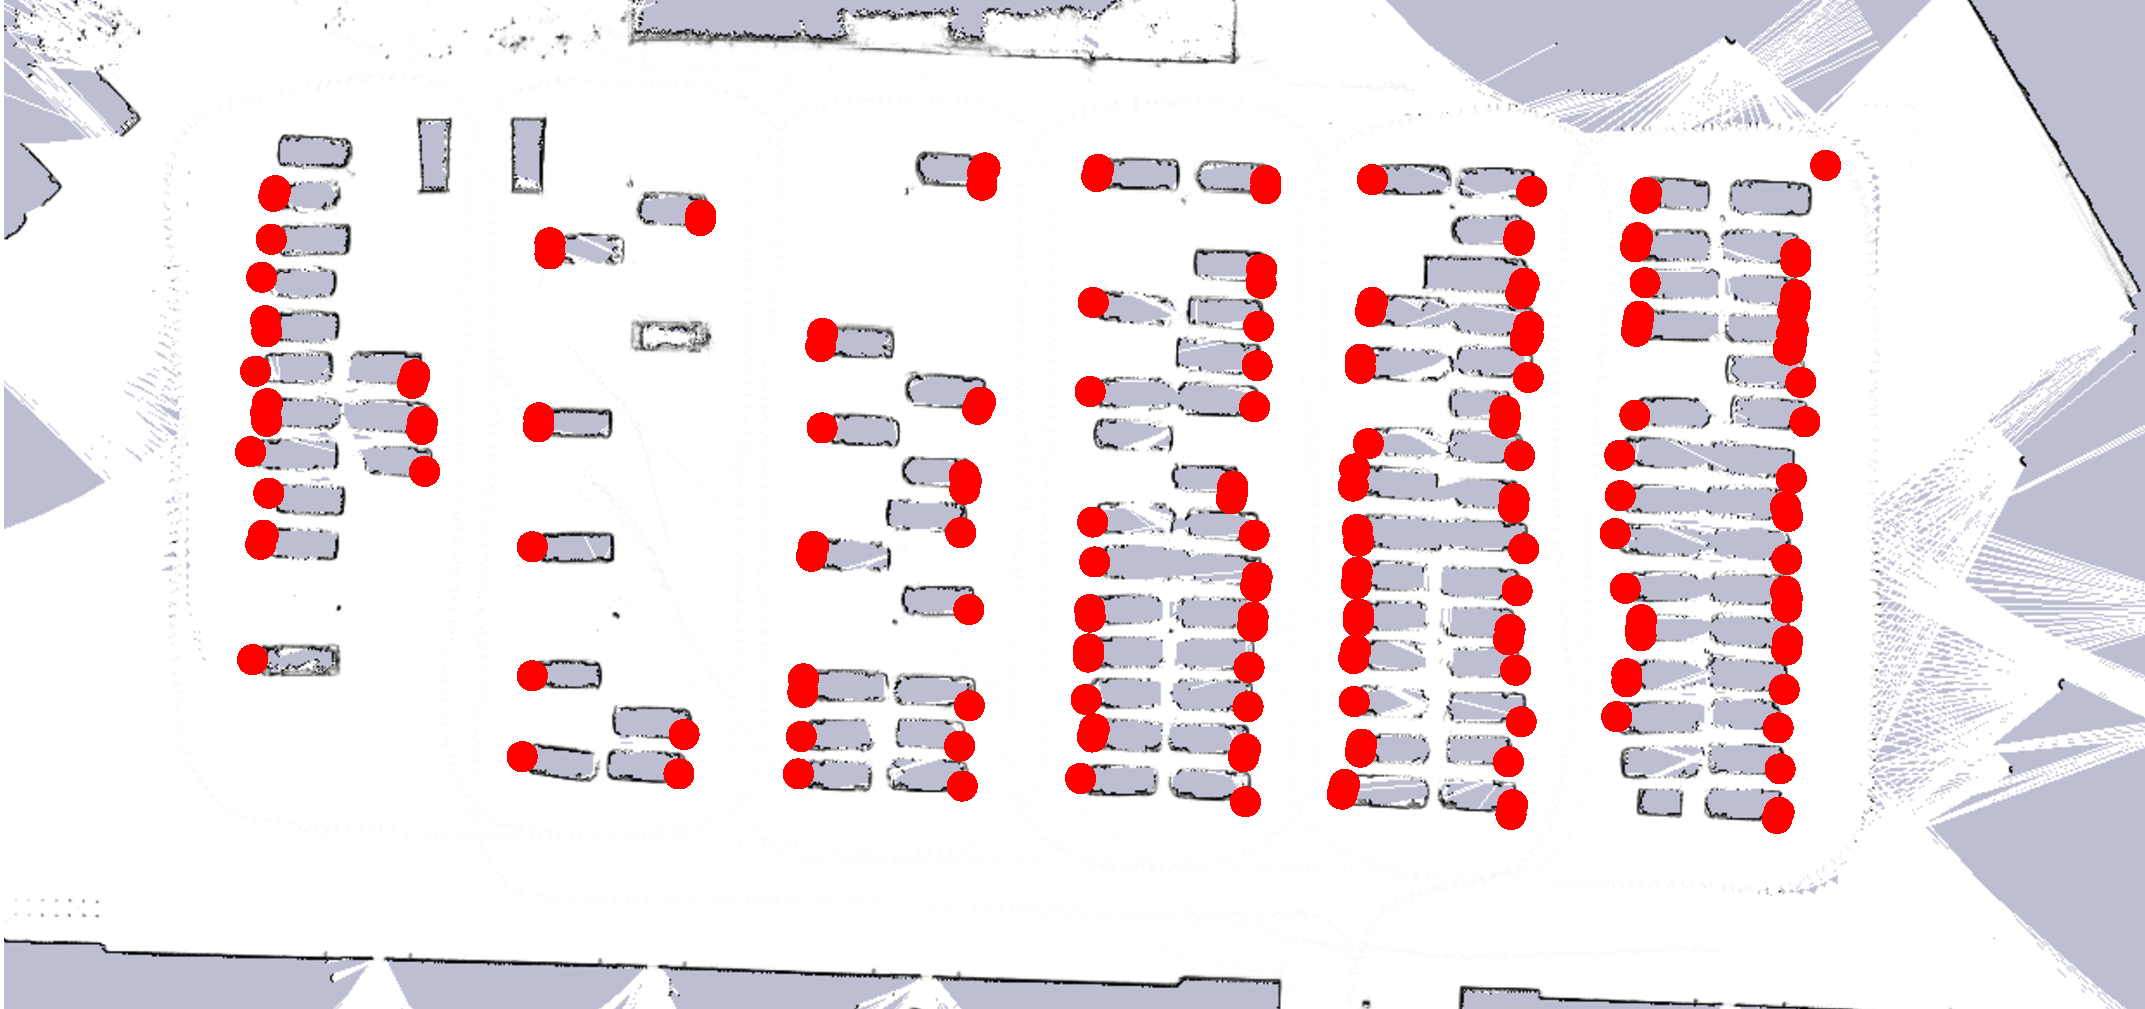
\includegraphics[width=0.47\textwidth]{pictures/laser_fusion_13_1.pdf}}\hspace{2mm}
\subfloat{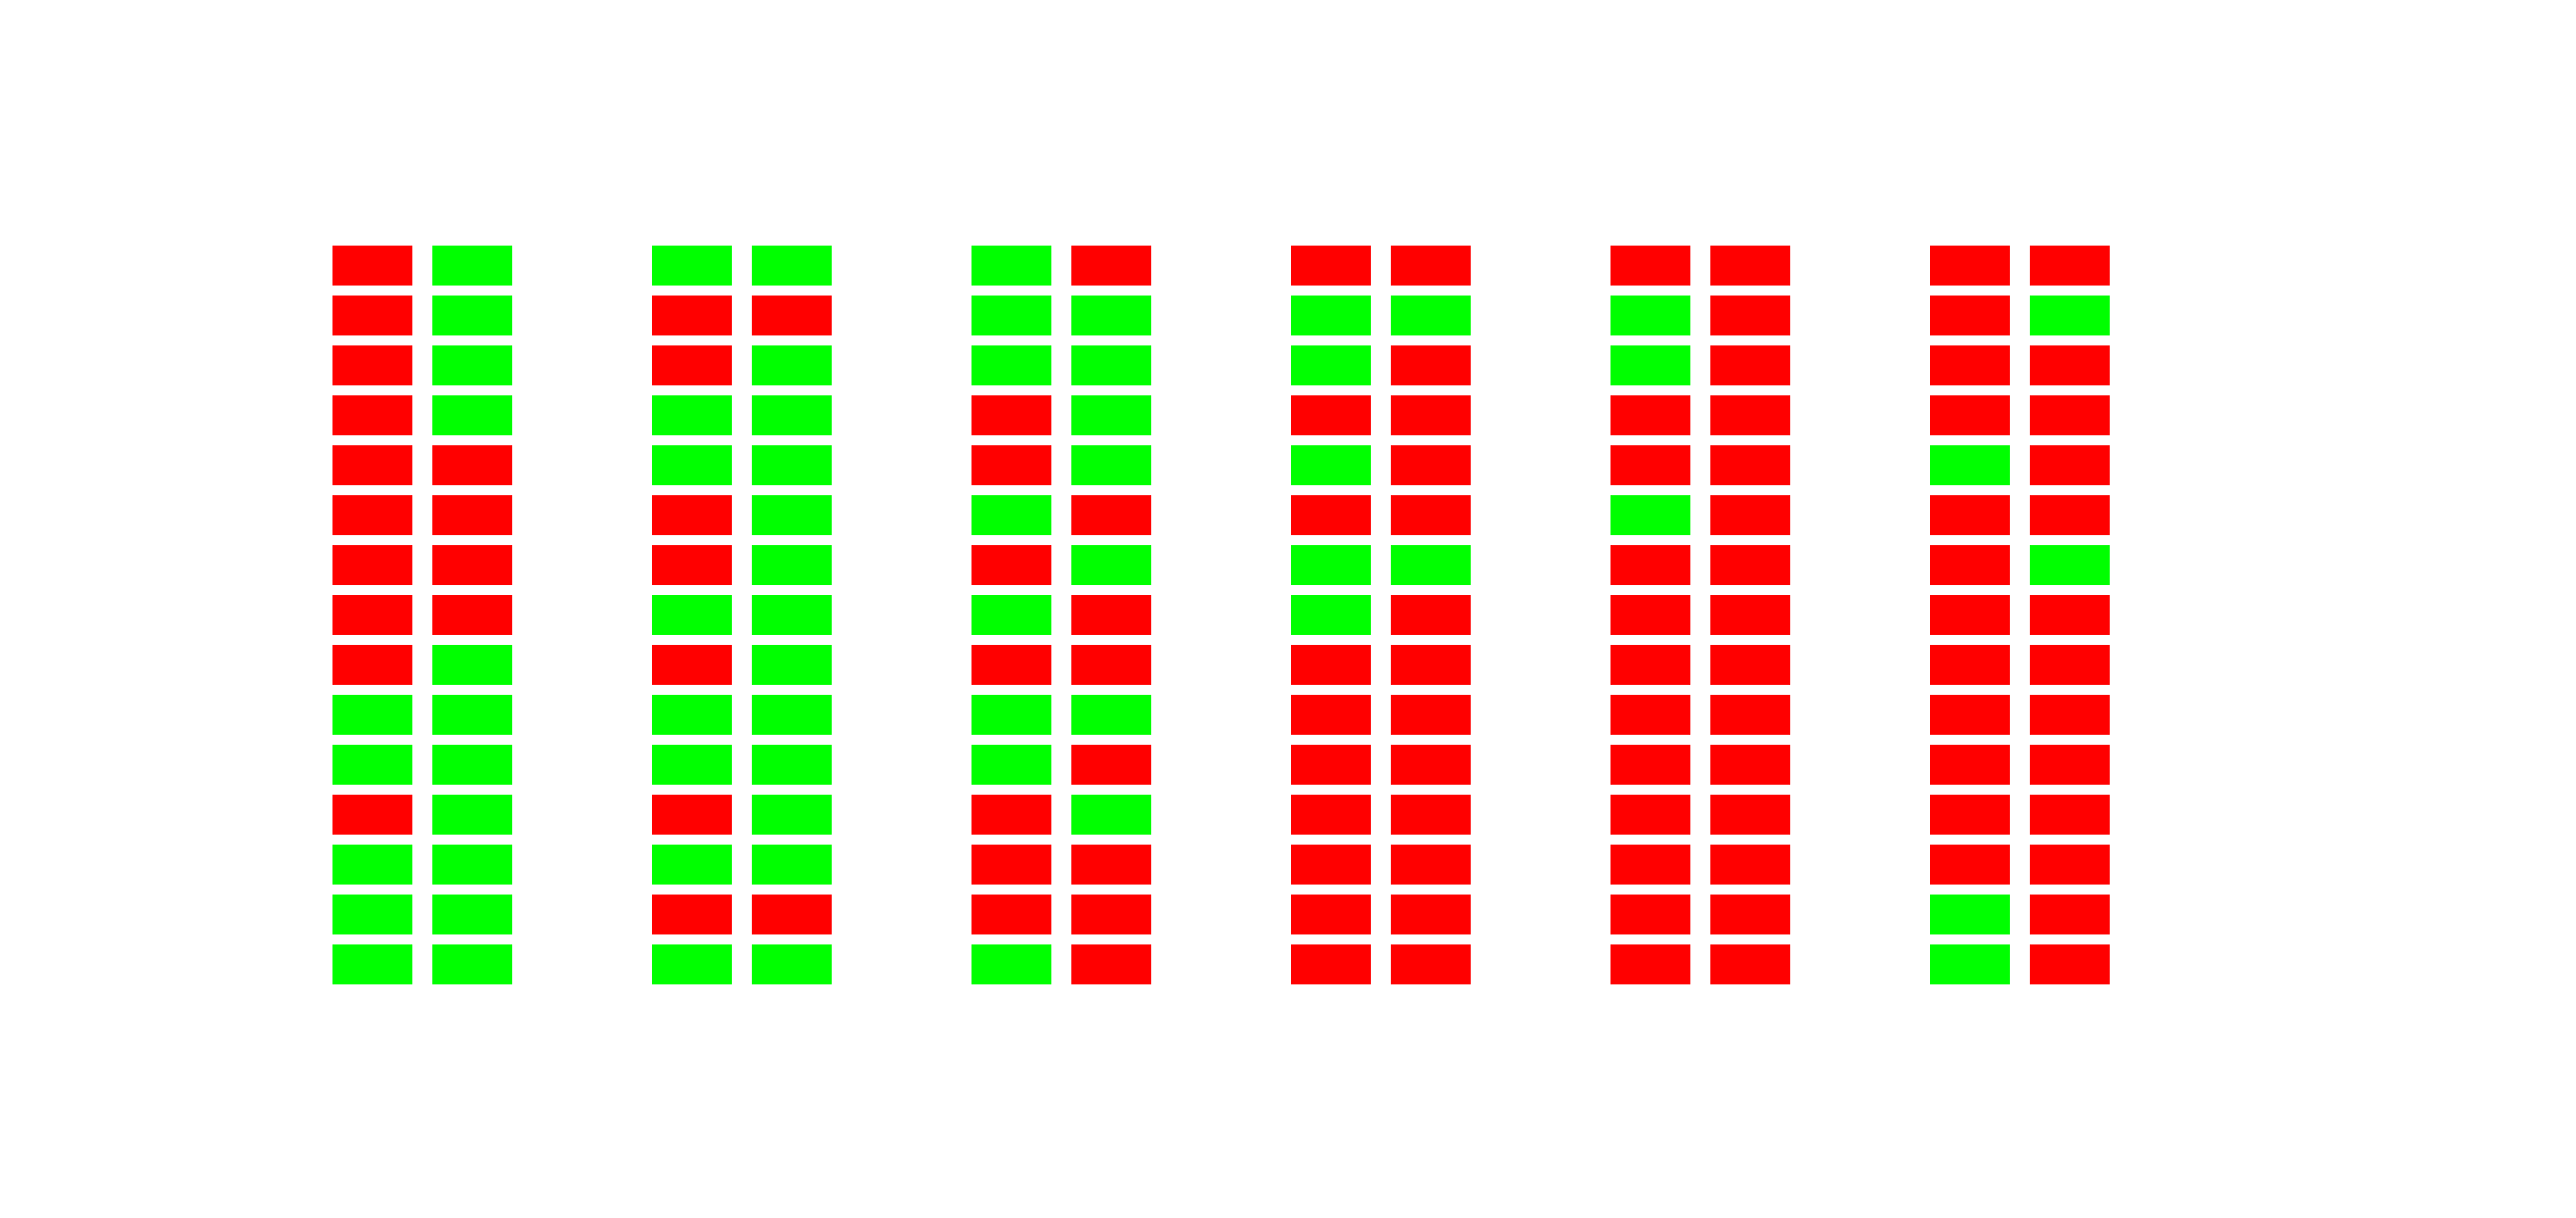
\includegraphics[width=0.47\textwidth]{pictures/parking_lots_13_1.png}}\\
\subfloat{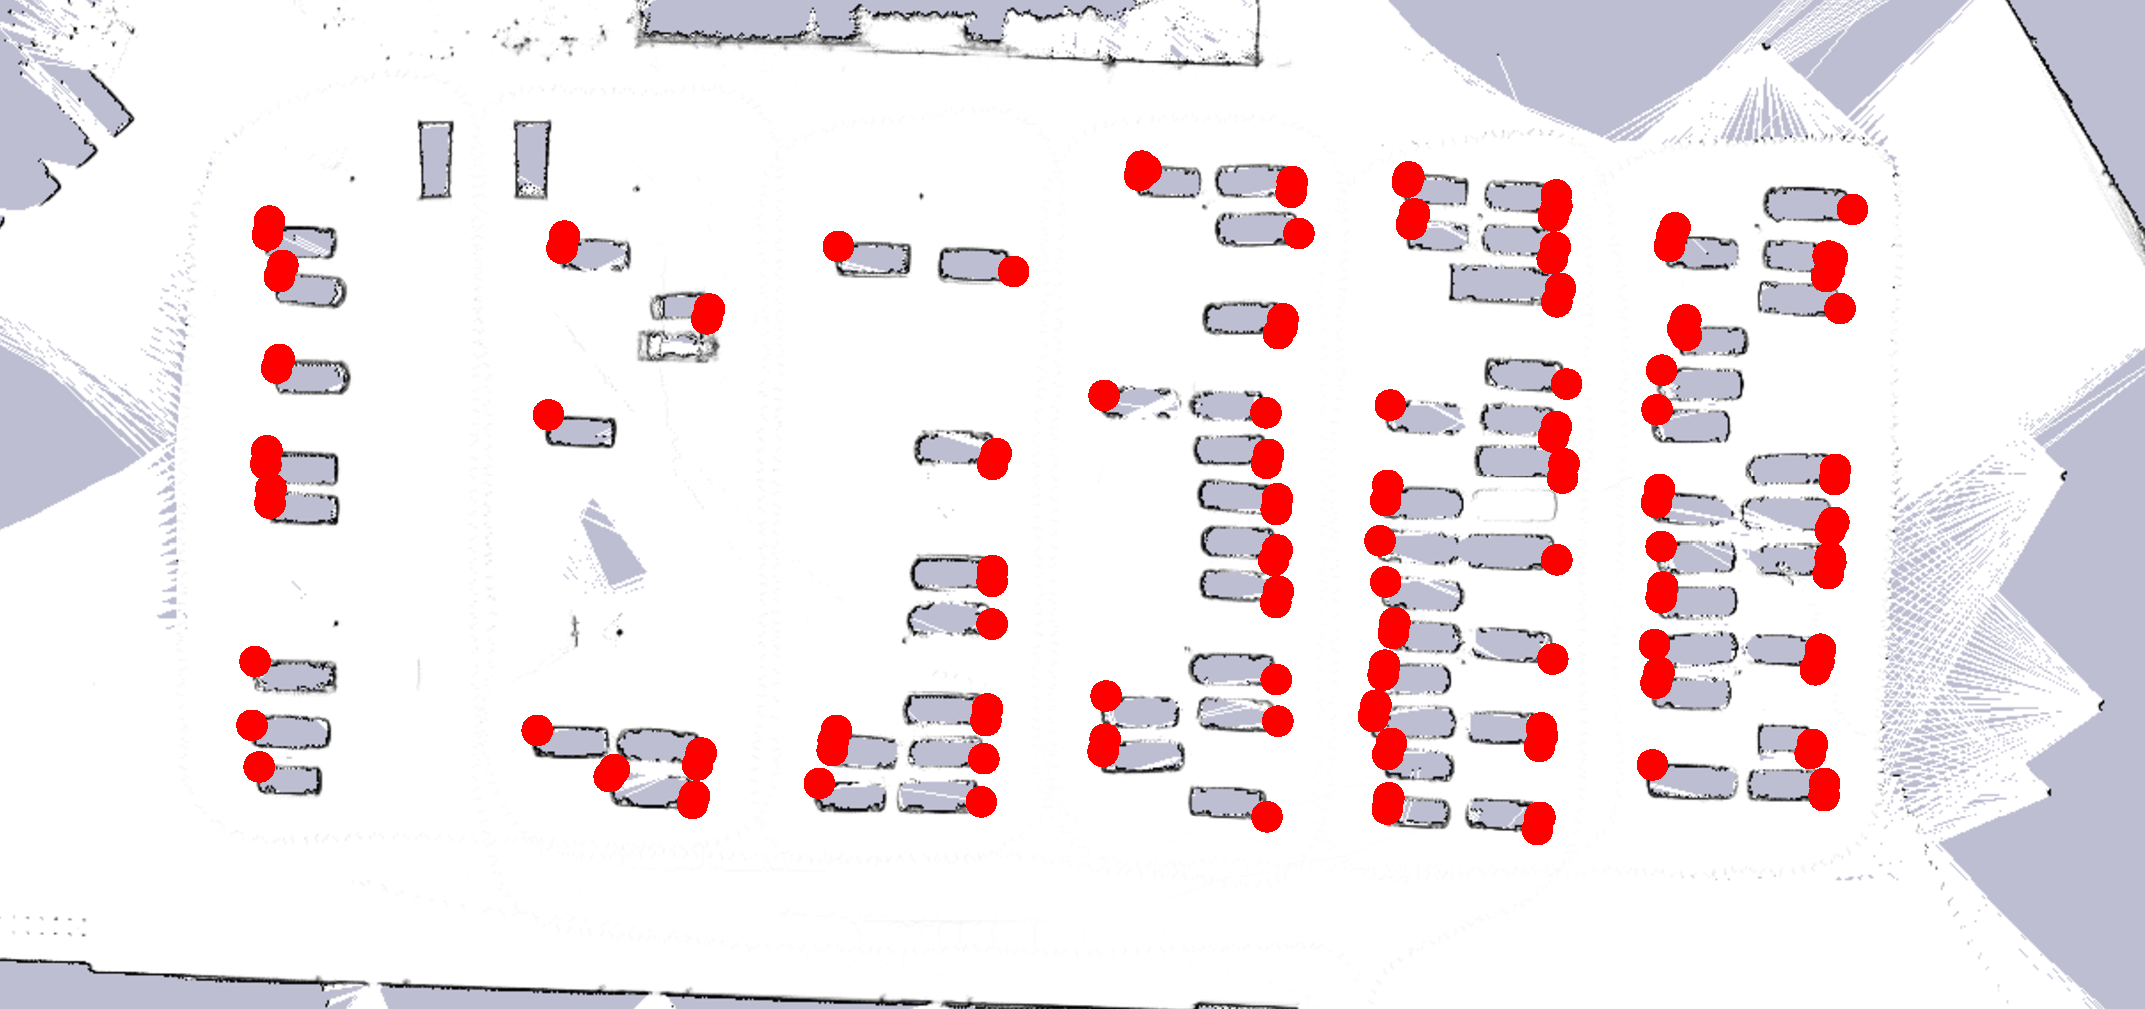
\includegraphics[width=0.47\textwidth]{pictures/laser_fusion_15_1.pdf}}\hspace{2mm}
\subfloat{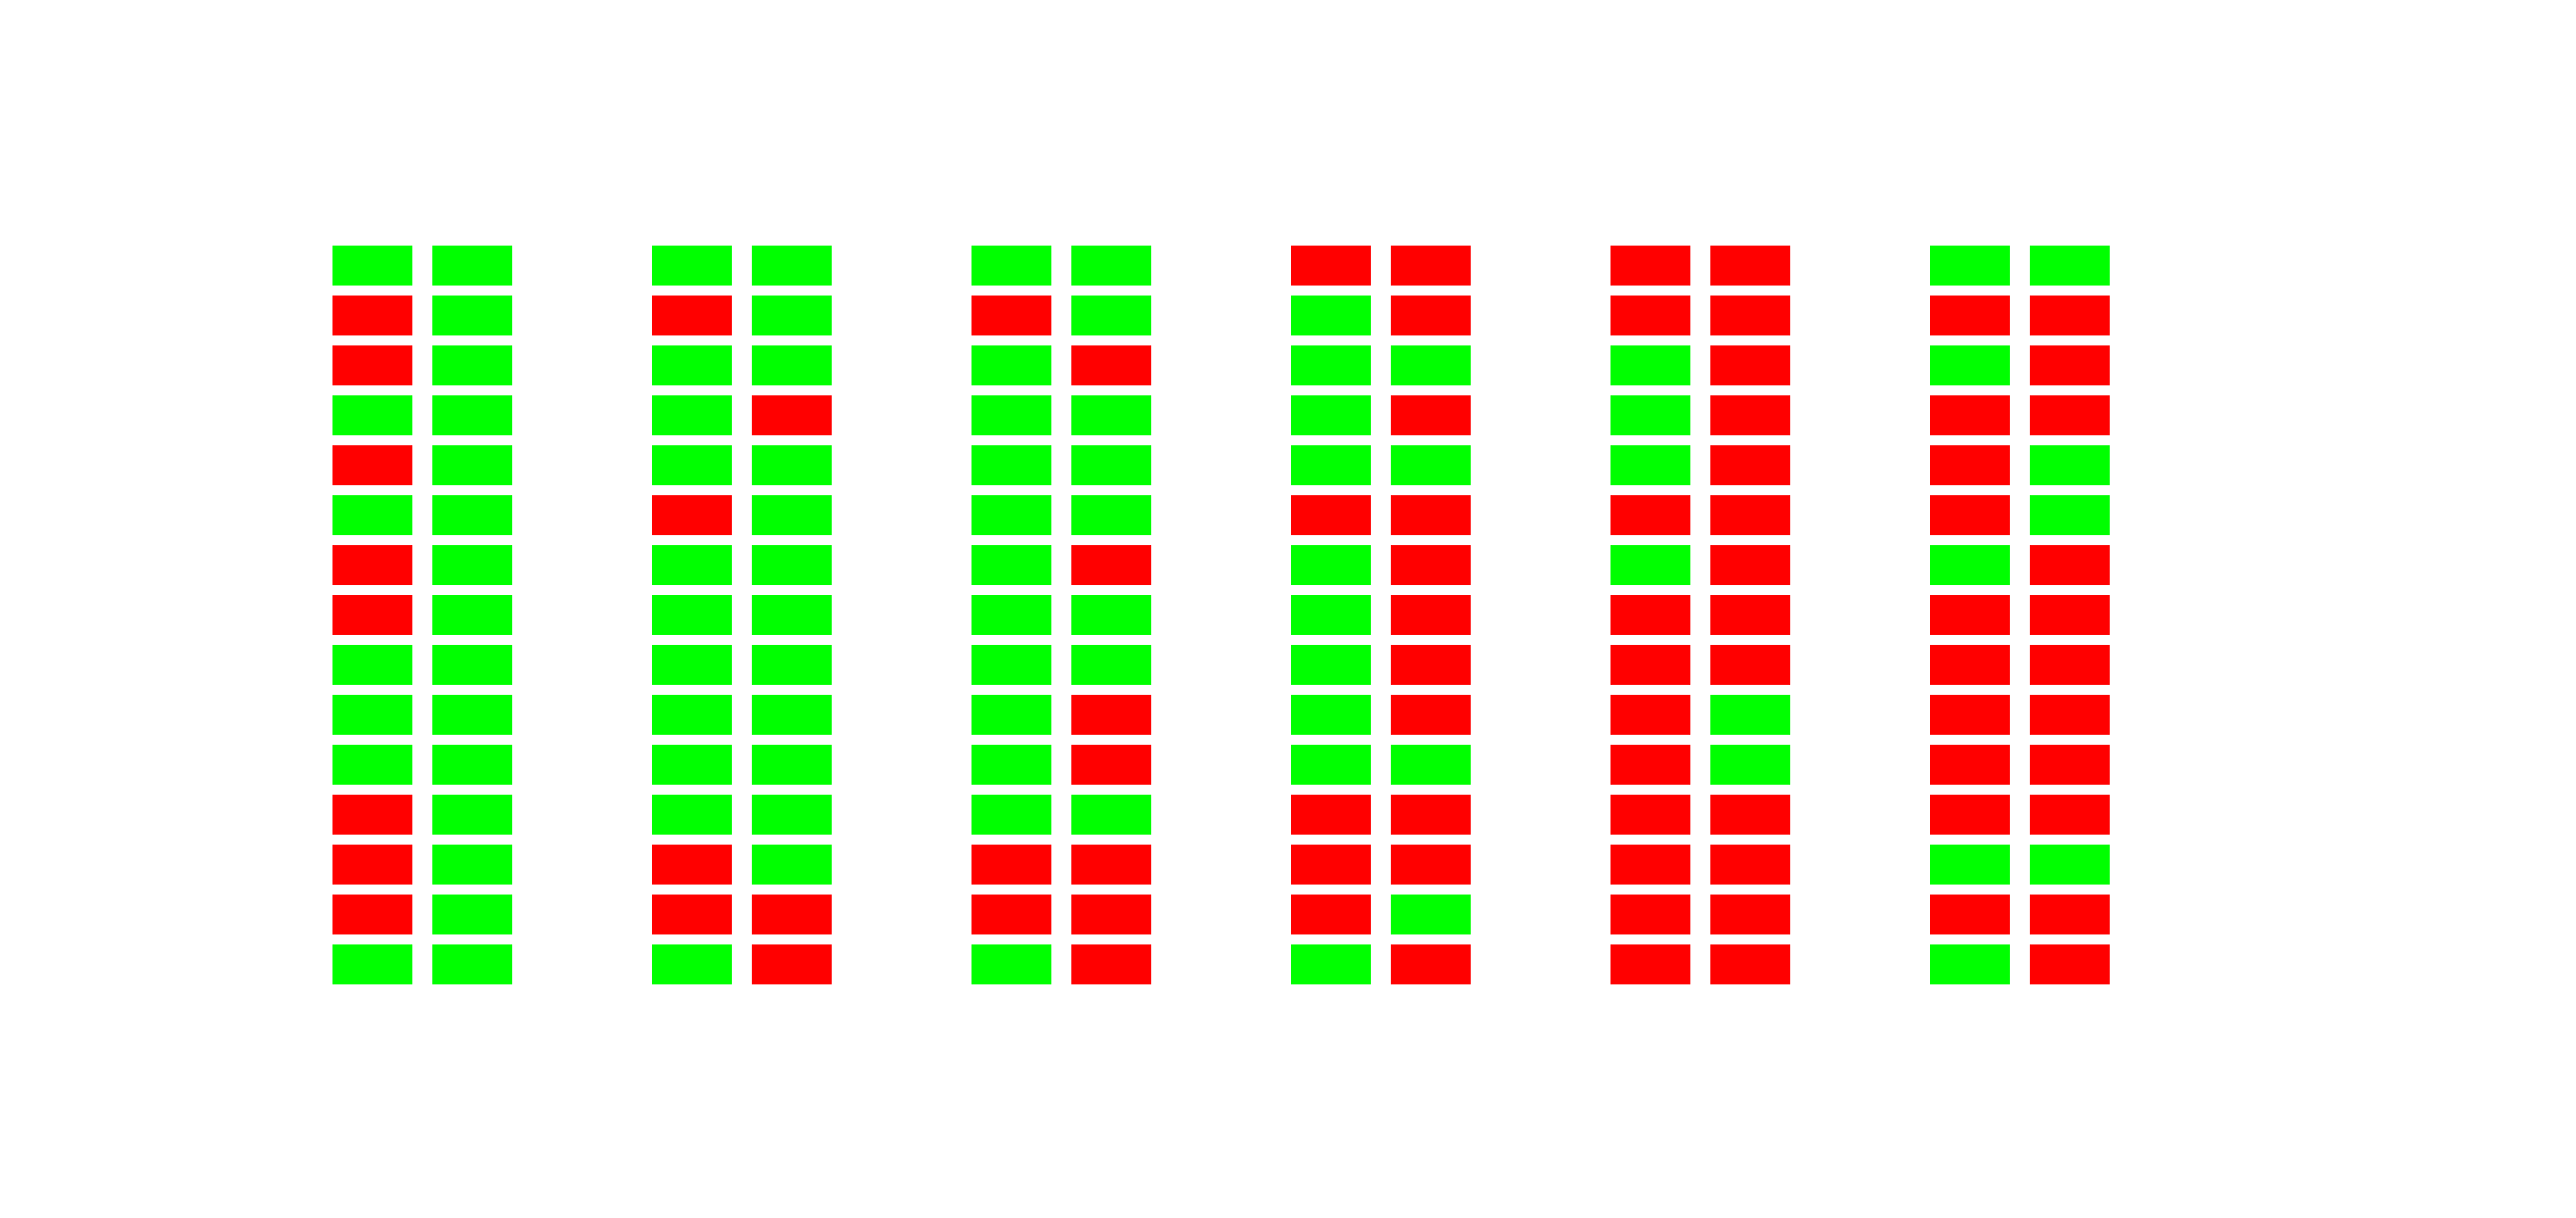
\includegraphics[width=0.47\textwidth]{pictures/parking_lots_15_1.png}}\\
\subfloat{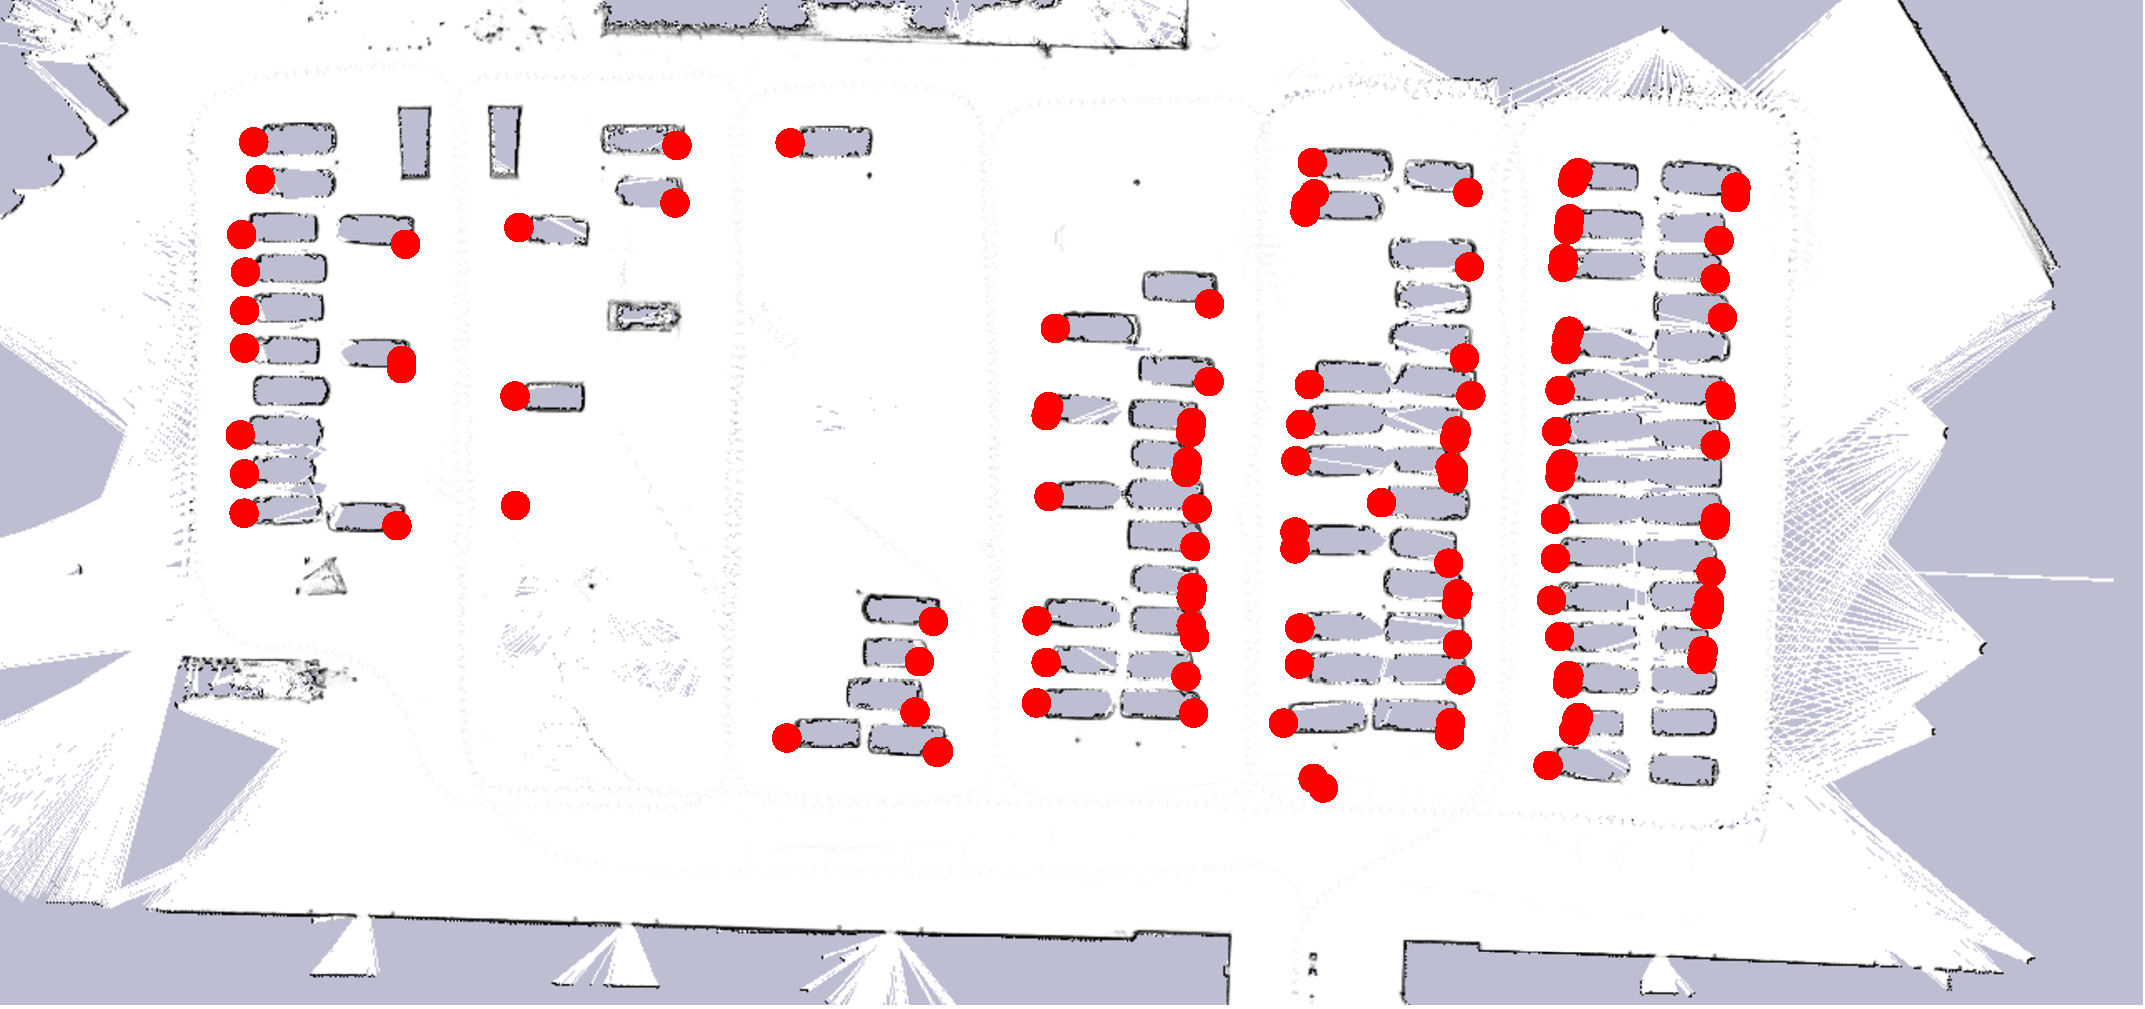
\includegraphics[width=0.47\textwidth]{pictures/laser_fusion_12_12.pdf}}\hspace{2mm}
\subfloat{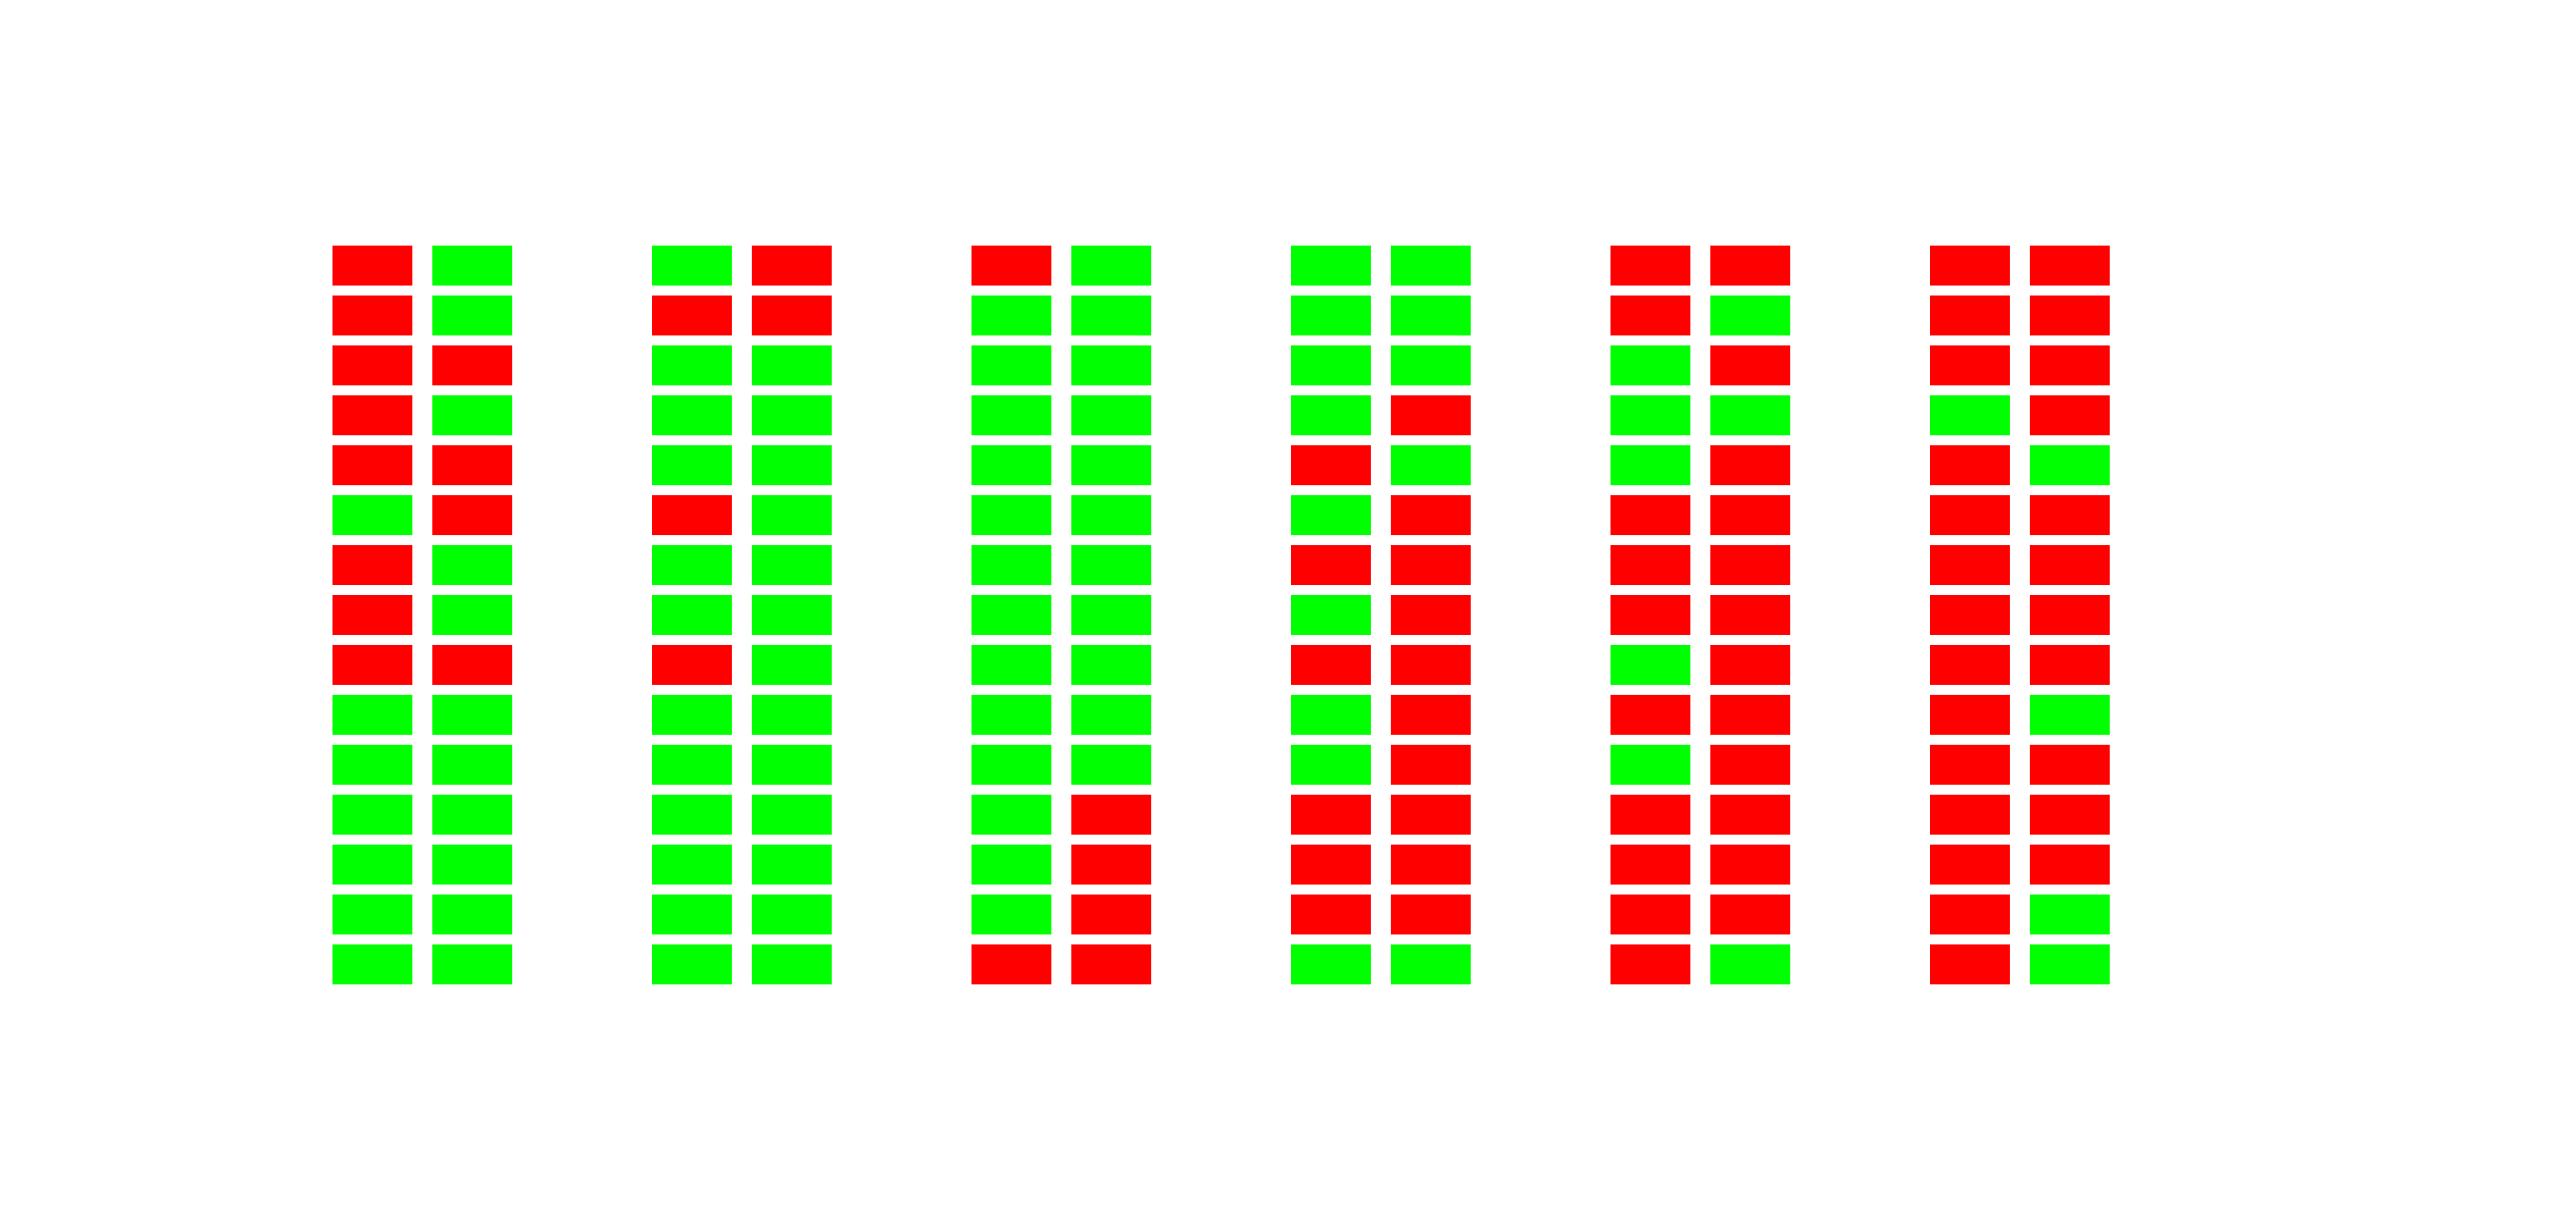
\includegraphics[width=0.47\textwidth]{pictures/parking_lots_12_12.png}}\\
\caption{Examples of detections of different cars under different light conditions.}
\label{fig:mapping_examples_1}
\end{figure}

\begin{figure}[p]%
\centering
\subfloat{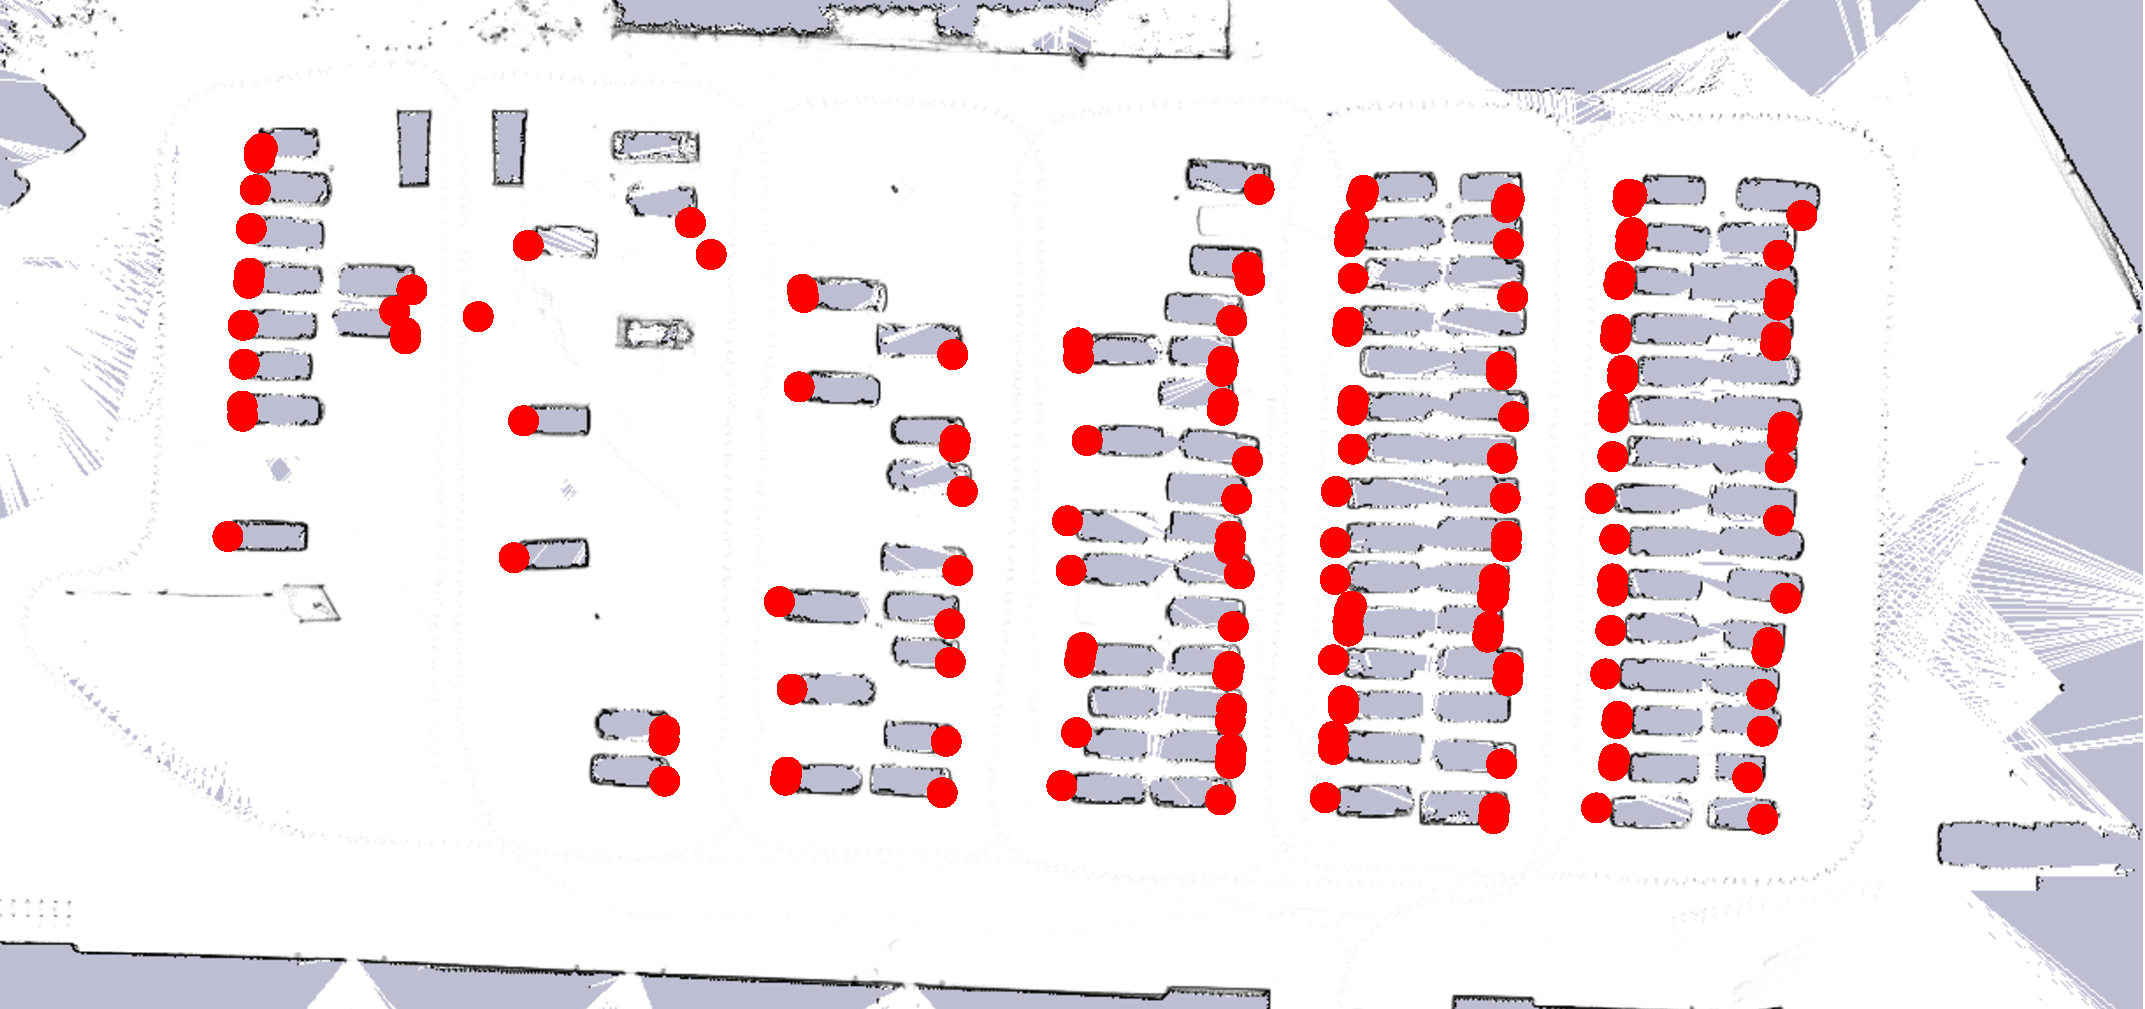
\includegraphics[width=0.47\textwidth]{pictures/laser_fusion_5_12.pdf}}\hspace{2mm}
\subfloat{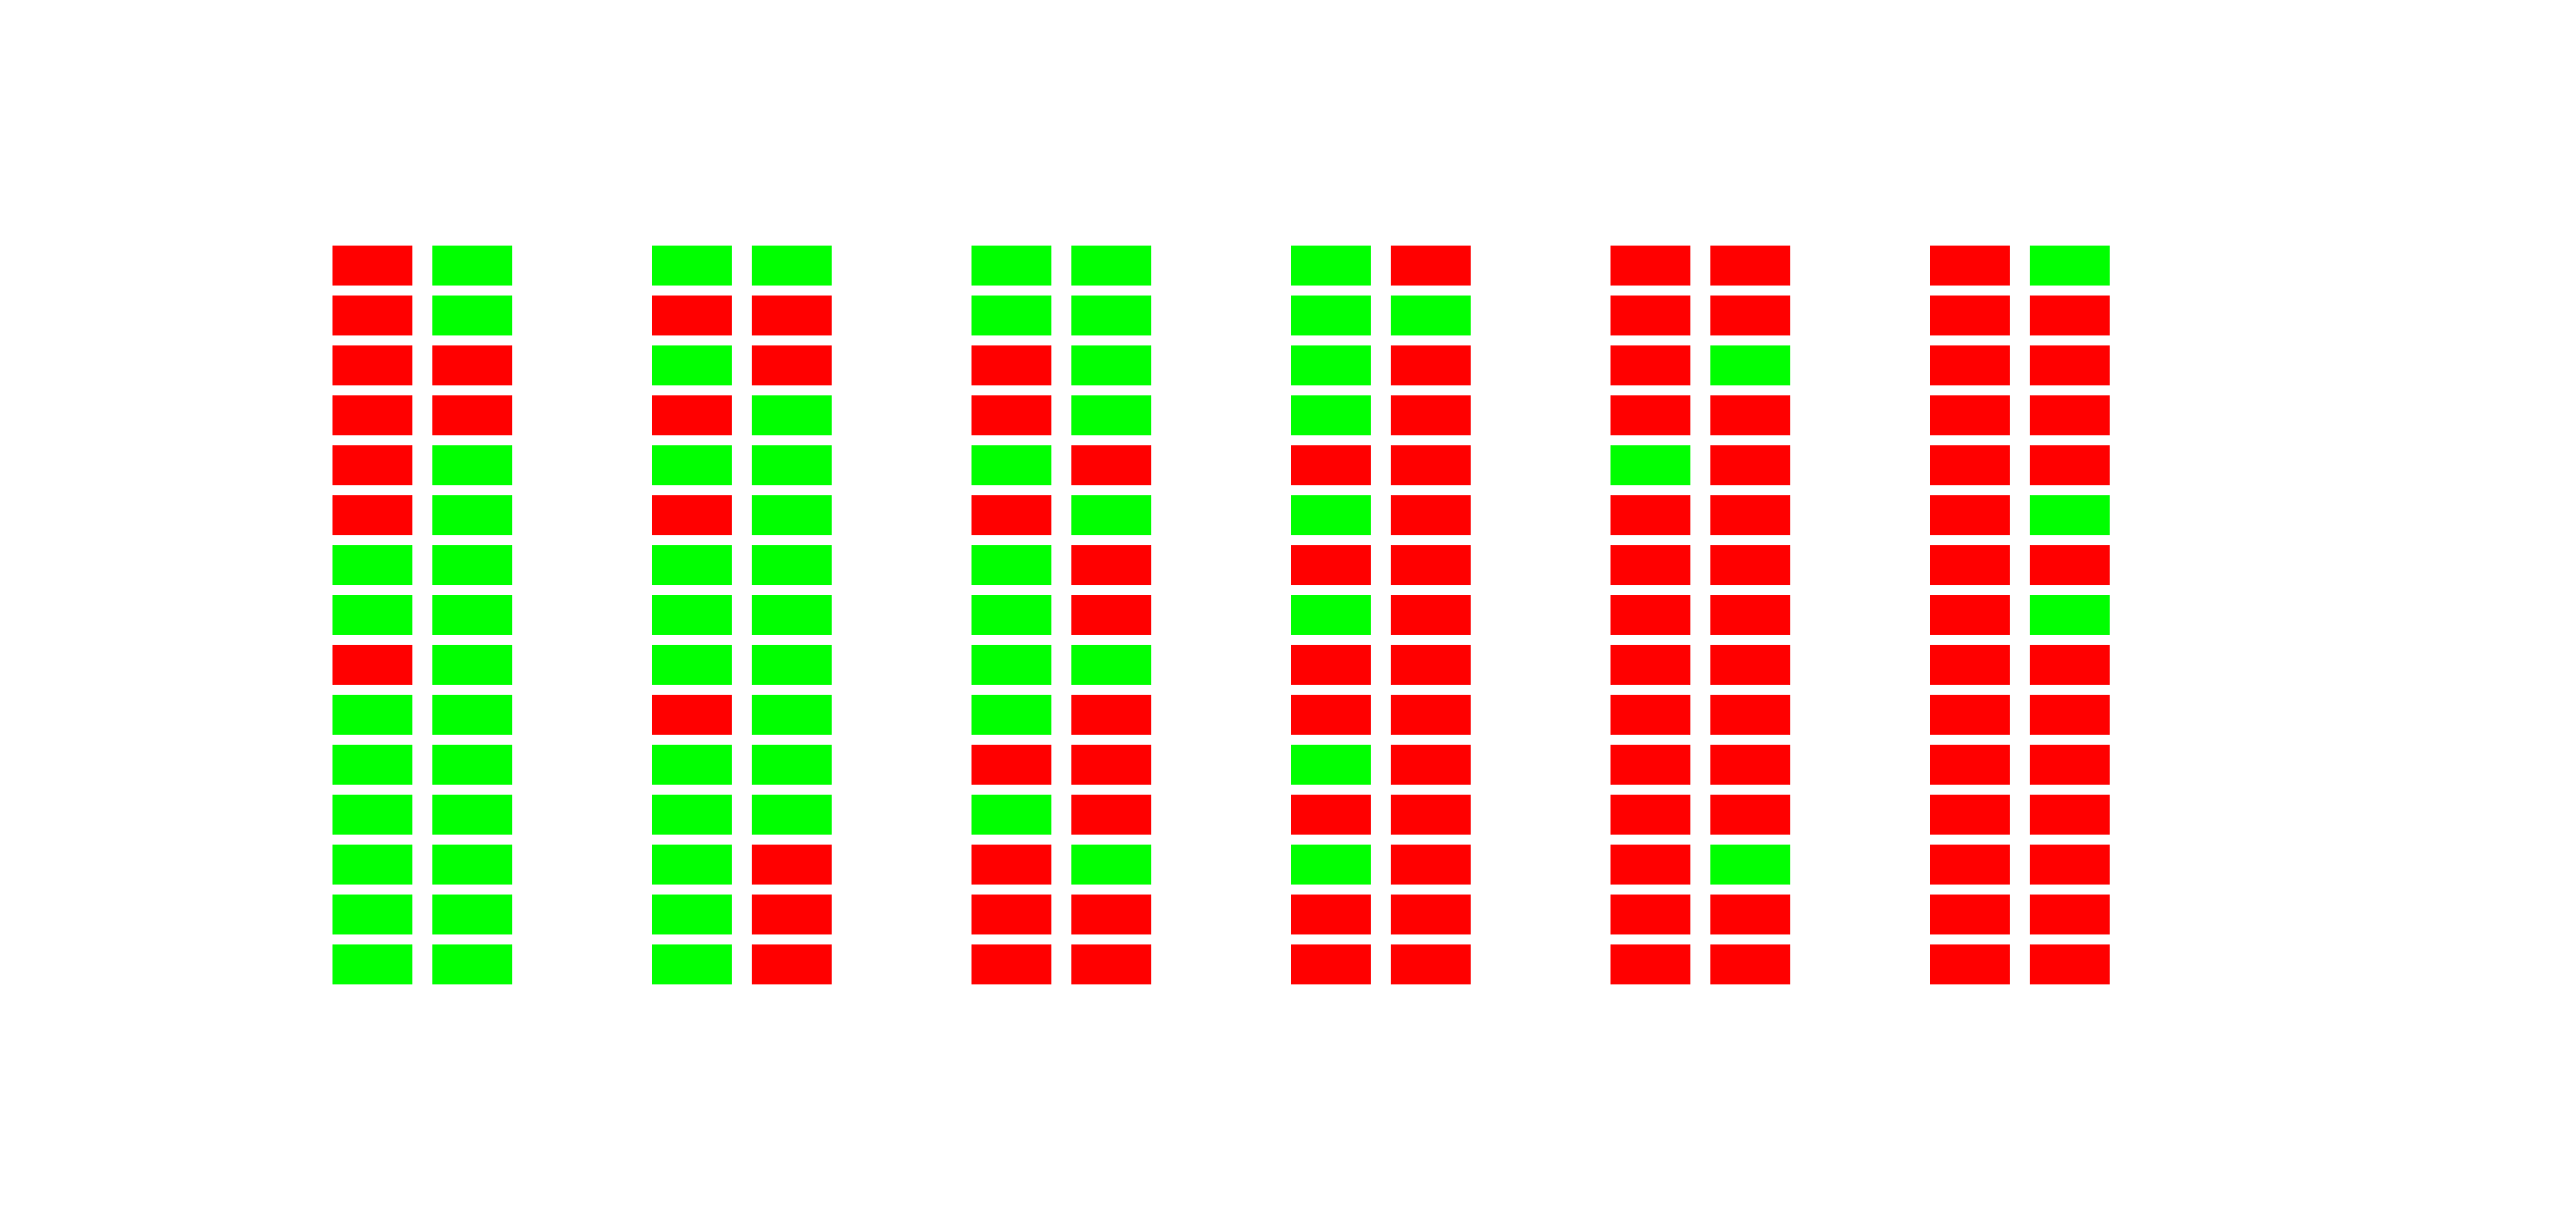
\includegraphics[width=0.47\textwidth]{pictures/parking_lots_5_12.png}}\\
\subfloat{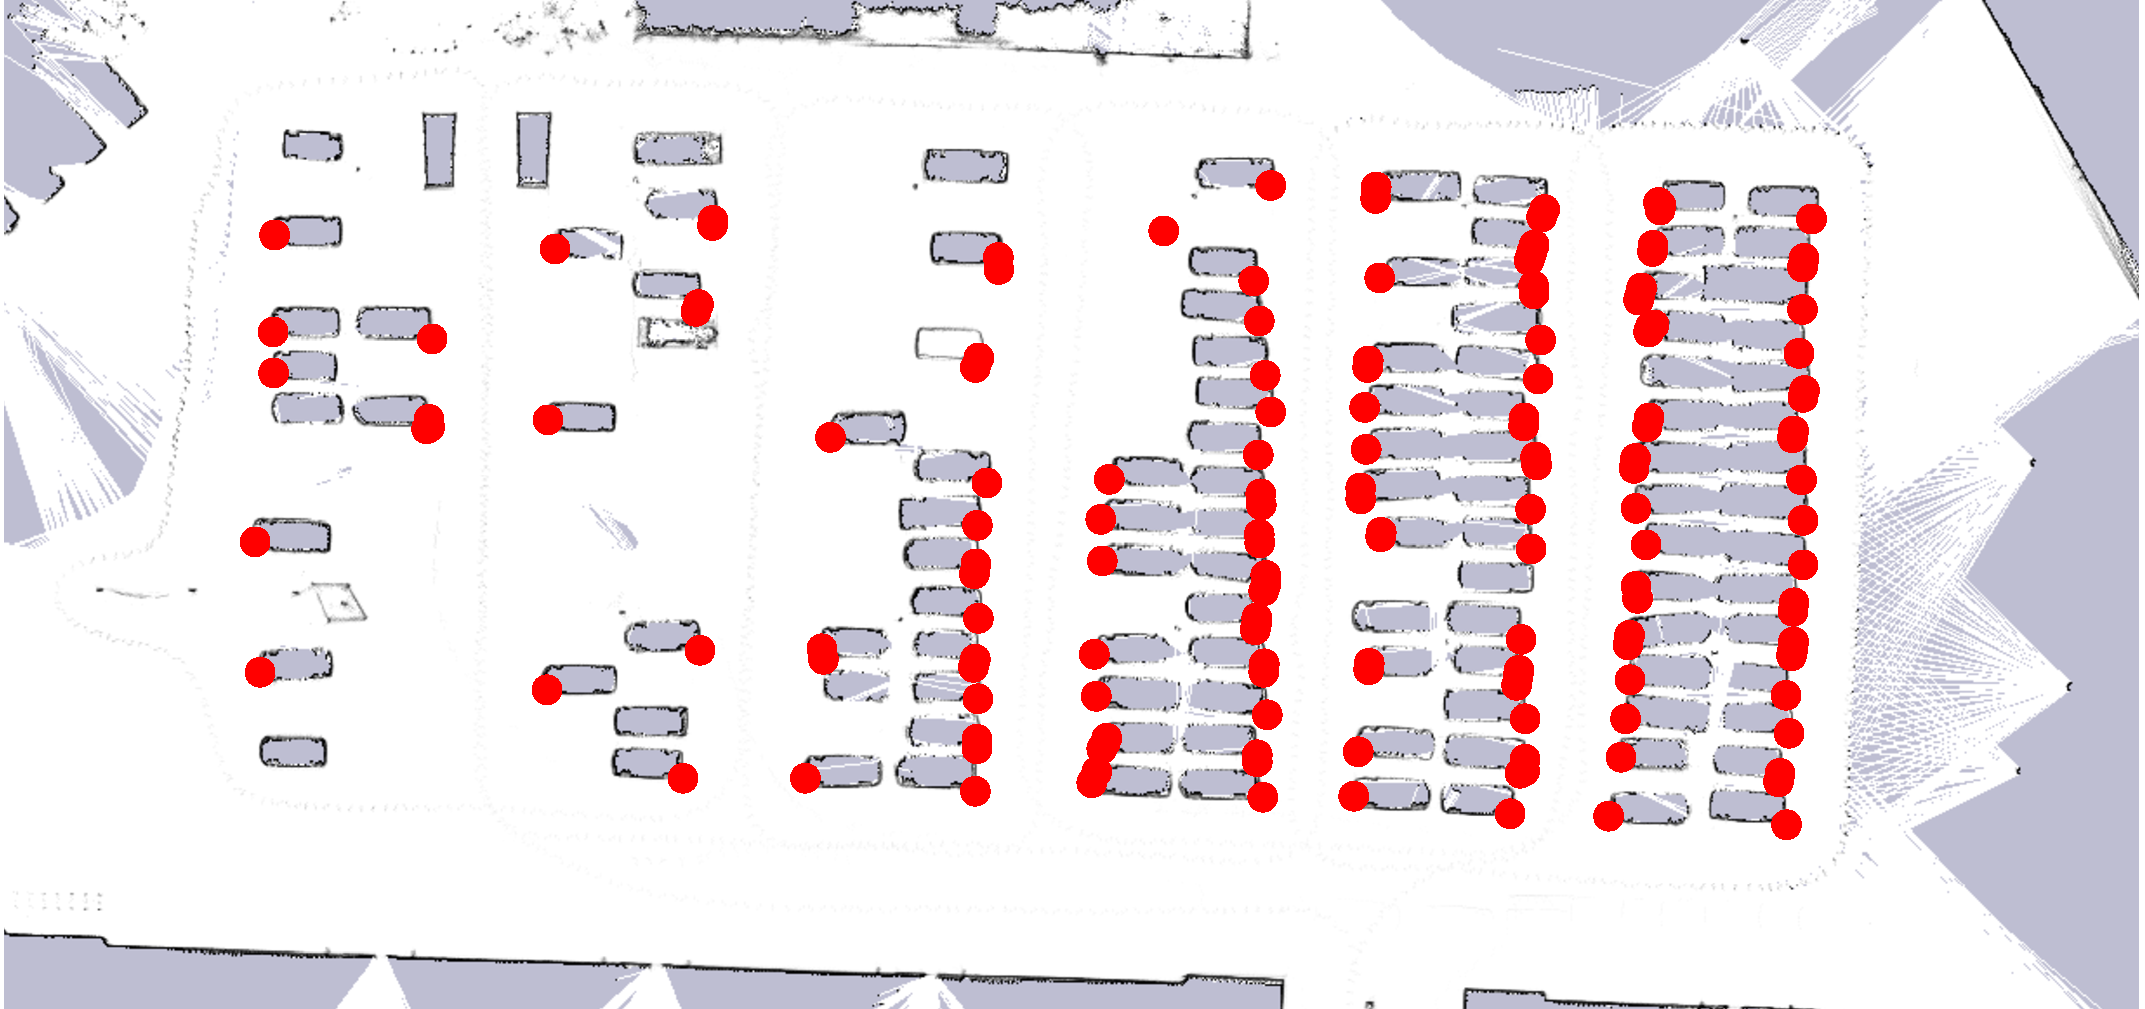
\includegraphics[width=0.47\textwidth]{pictures/laser_fusion_6_12.pdf}}\hspace{2mm}
\subfloat{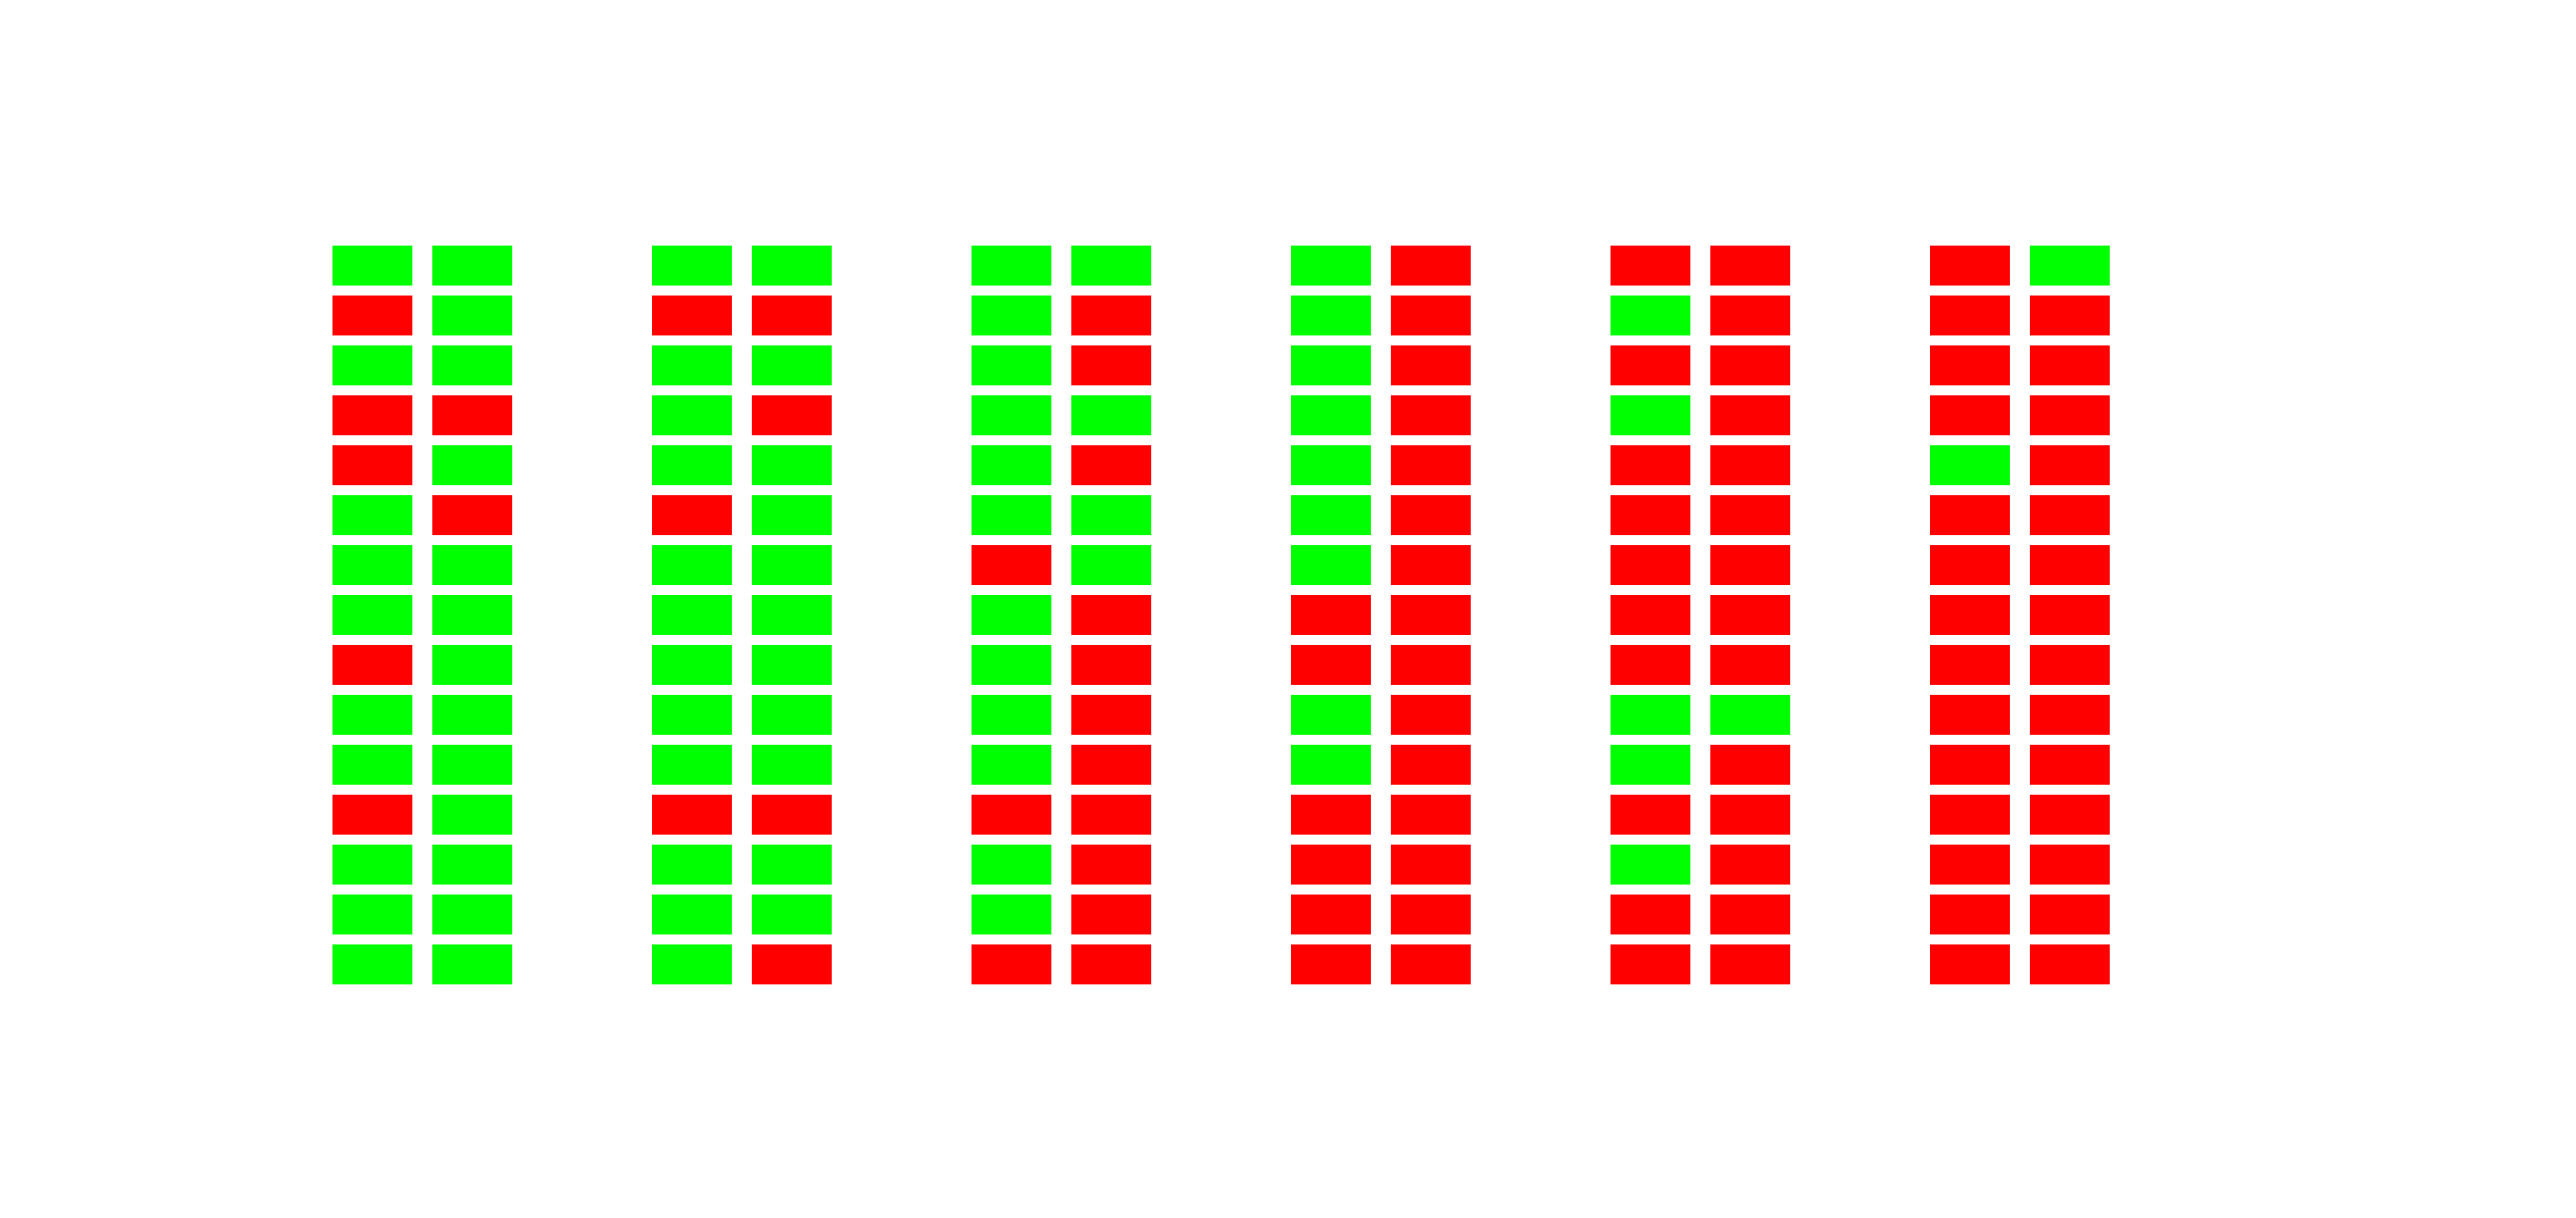
\includegraphics[width=0.47\textwidth]{pictures/parking_lots_6_12.png}}\\
\subfloat{\includegraphics[width=0.47\textwidth]{pictures/laser_fusion_9_12.pdf}}\hspace{2mm}
\subfloat{\includegraphics[width=0.47\textwidth]{pictures/parking_lots_9_12.png}}\\
\subfloat{\includegraphics[width=0.47\textwidth]{pictures/laser_fusion_11_12.pdf}}\hspace{2mm}
\subfloat{\includegraphics[width=0.47\textwidth]{pictures/parking_lots_11_12.png}}\\
\caption{Examples of detections of different cars under different light conditions.}
\label{fig:mapping_examples_2}
\end{figure}

Because of these issues, we mostly rely on the pre-defined positions of the
parking lots for occupancy estimation. An example of the occupancy information
from the data gathered during one run is presented in
Figure~\ref{subfig:pre_defined}. The exact positions of the parking lots and
deterministic association of detections to them allows us to quantify the
parking lot positions estimation precision. For this system we measure the
detection rate throughout the course of 21 data acquisition sessions. A
session is a sequence of measurements that provide the occupancy information
of every parking lot in the area of interest.
Figure~\ref{fig:mapping_examples_1} and Figure~\ref{fig:mapping_examples_2}
each show 4 examples of such sessions. We estimate the precision of parking
lot occupancy detection as a relation of the number of correctly labeled
parking lots to the total number of parking lots. This results in:
$\frac{\mathrm{correct}}{\mathrm{total}} \approx 90\% $ of all parking lots to
be labeled correctly as occupied or free respectively. The exact precision, if
calculated on the subset of sessions presented in
Figure~\ref{fig:mapping_examples_1} and Figure~\ref{fig:mapping_examples_2},
equals 90.83\% as a result of 132 wrongly labeled parking lots out of the
total number of 1440.

There are two main sources of errors. The first one is failing to detect the
cars or assigning them to the wrong parking lot. Failing to detect a car
logically propagates from the visual detection part. The data association
error is usually due to abnormal sizes of the cars or improper position in the
parking lot. The second source of error is an assumption that the world stays
static while the dataset is being acquired.

% section parking_lots_modeling (end)


\section{Action Planning}
\label{sec:planning_results}

\begin{figure}[t]
\begin{center}
\includegraphics[width=0.5\textwidth]{pictures/graph_observations.pdf}
\end{center}
\caption{A visual representation of the parking lot graph useful for planner visualization. The edges are defined similarly to~\ref{fig:graph}. Each state contains prediction and observation information. This can be seen as combining occupancy information in Figure~\ref{subfig:pre_defined} with Figure~\ref{fig:occupancy_accumulated}.}
\label{fig:graph_accumulated_illustration}
\end{figure}


\begin{figure}[t]
\begin{center}
\subfloat[]{\includegraphics[width=0.4\textwidth]{pictures/walk_4_drive_10_wait_10_data_log_12_12_2013_states.pdf}}\hspace{2mm}
\subfloat[]{\includegraphics[width=0.4\textwidth]{pictures/walk_4_drive_10_wait_10_data_log_12_12_2013_path_1.pdf}}\hspace{2mm}
\end{center}
\caption{An optimal strategy for $v_{\mathrm{walk}} = 4$ km/h, $v_{\mathrm{drive}} = 10$ km/h and the failure cost of 10 seconds. Each state is presented by an inner and an outer circles. The inner circle depicts the real occupancy status on the day the experiment was held. The outer one presents the occupancy estimate based on the data accumulated from multiple runs. Both circle's colors vary from red for occupied parking lots to green for free ones.}
\label{fig:w_4_d_10_w_10_log_12_12}
\end{figure}

\begin{figure}[b]%
\centering
\subfloat[Drive up.]{\includegraphics[width=0.15\textwidth]{pictures/action_up.pdf}}\hspace{2mm}
\subfloat[Drive right.]{\includegraphics[width=0.15\textwidth]{pictures/action_right.pdf}}\hspace{2mm}
\subfloat[Drive down.]{\includegraphics[width=0.15\textwidth]{pictures/action_down.pdf}}\hspace{2mm}
\subfloat[Drive left.]{\includegraphics[width=0.15\textwidth]{pictures/action_left.pdf}}\hspace{2mm}
\subfloat[Try to park.]{\includegraphics[width=0.15\textwidth]{pictures/action_park.pdf}}
\caption{Visualization of the actions considered optimal by a policy on the graph.}
\label{fig:actions}
\end{figure}

In this section we present the evaluation of the work of the MDP based
planner, that searches for a free parking space. As a testing environment we
use the parking lot at the campus of the University of Freiburg.

We make use of the occupancy information gathered from integrating the
measurements of the parking lots' occupancy (see
Figure~\ref{subfig:pre_defined}) as observed during a period of 21 days. In
order to be able to show the results of the planner we introduce a number of
visualizations. We visualize every parking space as a state in which the agent
can perform an action to park as presented in
Figure~\ref{fig:graph_accumulated_illustration}, where each state shows both
--- the prediction of the occupancy probability as an outer circle and the
actual free or occupied state as the inner one. This representation is useful
to see in a glance what the state of the parking was on the specific date,
while being able to analyze the reasoning behind the agent's actions. However,
only the information shown as an outer circle --- the occupancy prediction is
available to the robot on the planning step. The occupancy prediction is only
then updated to the real occupancy status, when the parking lot is observed by
the agent as he drives by. The actions, that the agent is able to carry out,
as presented in~\eqref{eq:actions} are visualized in the way shown in
Figure~\ref{fig:actions}.


As described in Section~\ref{sec:action_planning} there are 3 core parameters
that influence the performance of the planner: $v_{\mathrm{walk}}$, $v_{\mathrm{drive}}$ and the
failure cost. In this section we present the differences in the behavior of
the agent with respect to different values of these parameters. All the
experiments share the same actual positions of the parked cars for the ease of
comparison.

For these parameters we consider a number of sets of their values. We further
present the differences in the approach picked by the agent depending on the
different sets of the parameters.

\begin{figure}[t]
\begin{center}
\vspace{-5mm}
\subfloat[Initial parking lot state.]{\includegraphics[width=0.35\textwidth]{pictures/walk_4_drive_10_wait_90_data_artificial_states.pdf}}\hspace{2mm}
\subfloat[$1^{st}$ iteration.]{\includegraphics[width=0.35\textwidth]{pictures/walk_4_drive_10_wait_90_data_artificial_path_1.pdf}}\\\vspace{-5mm}
\subfloat[$2^{nd}$ iteration.]{\includegraphics[width=0.35\textwidth]{pictures/walk_4_drive_10_wait_90_data_artificial_path_2.pdf}}\hspace{2mm}
\subfloat[$3^{rd}$ iteration.]{\includegraphics[width=0.35\textwidth]{pictures/walk_4_drive_10_wait_90_data_artificial_path_3.pdf}}\\\vspace{-5mm}
\end{center}
\caption{An optimal strategy for $v_{\mathrm{walk}} = 4$ km/h, $v_{\mathrm{drive}} = 10$ km/h and the failure cost of 90 seconds carried out on an artificial dataset.}
\label{fig:w_4_d_10_w_90_artificial}
\end{figure}

Figure~\ref{fig:w_4_d_10_w_10_log_12_12} shows the path considered optimal by
the agent, given the driving speed of 10 km/h and walking speed of 4 km/h.
Additionally, a failure cost of 10 seconds ensures, that the agent considers
that it loses 10 seconds for every unsuccessful parking action. This results
in the strategy that finds a trade-off between the distance from the parking
lots to the goal and their occupancy. The figure shows that the agent decides
for a state that combines close proximity to the goal state with locally high
probability of being free.

\begin{figure}[t]
\begin{center}
\subfloat[Optimal strategy for $v_{\mathrm{walk}} = 4$ km/h, $v_{\mathrm{drive}} = 10$ km/h and the failure cost of 90 seconds tested on the real data.]{\includegraphics[width=0.40\textwidth]{pictures/walk_2_drive_15_wait_90_data_log_12_12_2013_path_1.pdf}\label{subfig:long_wait_real}}\hspace{6mm}
\subfloat[Optimal strategy for $v_{\mathrm{walk}} = 10$ km/h, $v_{\mathrm{drive}} = 10$ km/h and the failure cost of 90 seconds tested on the real data.]{\includegraphics[width=0.40\textwidth]{pictures/walk_10_drive_10_wait_90_data_log_12_12_2013_path_1.pdf}\label{subfig:fast_walk}}
\end{center}
\caption{}
\label{fig:long_wait_fast_walk}
\end{figure}

Looking at Figure~\ref{fig:w_4_d_10_w_10_artificial} that shows the
performance of the search with the same core parameters on the artificial
dataset we see, that in a rare case of extremely high abnormal occupancy in
the area, the agent is too confident that the parking action would succeed and
it results in extremely long paths and numerous re-planning steps. The agent
tends to pick the places, situated closer to the goal. To deal with this issue
we set the failure cost to a high value, which results in penalizing the
choice of the parking lots in which the agent is likely to fail the parking
action. Setting the failure cost to 90 seconds results in a much more
conservative behavior as presented in
Figure~\ref{fig:w_4_d_10_w_90_artificial}.

Such conservative strategy also proves to be efficient in the real world
scenarios as can be seen in Figure~\ref{subfig:long_wait_real}, showing only a
rare need for re-planning. However, this strategy keeps the agent from making
overly optimistic decisions and he hardly ever observes the most occupied
parts of the parking lot.

Another interesting example that is worth mentioning is the test where human
speed is set to a high value. In the Figure~\ref{subfig:fast_walk} we observe,
that the agent makes the decision that the most practical strategy is to park
in the closest to the starting state parking space and walk to the goal from
there. This is a result of setting $v_{\mathrm{walk}}$ to be equal to $v_{\mathrm{drive}}$. It
may be explained as follows: if the walking speed is equal to the driving
speed it makes no sense driving around the parking lot when it is possible to
walk straight to the goal.


\begin{figure}[tbh]
\begin{center}
\subfloat[Initial parking lot state.]{\includegraphics[width=0.40\textwidth]{pictures/walk_4_drive_10_wait_10_data_artificial_states.pdf}}\hspace{2mm}
\subfloat[$1^{st}$ iteration.]{\includegraphics[width=0.40\textwidth]{pictures/walk_4_drive_10_wait_10_data_artificial_path_1.pdf}}\\
\subfloat[$3^{rd}$ iteration.]{\includegraphics[width=0.40\textwidth]{pictures/walk_4_drive_10_wait_10_data_artificial_path_3.pdf}}\hspace{2mm}
\subfloat[$4^{th}$ iteration.]{\includegraphics[width=0.40\textwidth]{pictures/walk_4_drive_10_wait_10_data_artificial_path_4.pdf}}\\
\subfloat[$16^{th}$ iteration.]{\includegraphics[width=0.40\textwidth]{pictures/walk_4_drive_10_wait_10_data_artificial_path_16.pdf}}\hspace{2mm}
\subfloat[$22^{nd}$ iteration.]{\includegraphics[width=0.40\textwidth]{pictures/walk_4_drive_10_wait_10_data_artificial_path_22.pdf}}
\end{center}
\caption{An optimal strategy for $v_{\mathrm{walk}} = 4$ km/h, $v_{\mathrm{drive}} = 10$ km/h and the failure cost of 10 seconds carried out on an artificial dataset.}
\label{fig:w_4_d_10_w_10_artificial}
\end{figure}
% section planning_results (end)
% chapter experimental_results (end)

